\section{分子结构基础 · 超级充实版}\label{ux5206ux5b50ux7ed3ux6784ux57faux7840-ux8d85ux7ea7ux5145ux5b9eux7248}

\textbf{📋 专题页}：03-专题/专题-分子结构基础（核心结论+对比表+例题）
\textbf{🔗 关联知识点}：Lewis结构式 · VSEPR理论 · 杂化轨道理论 · 离域π键 · 等电子体 · 分子轨道理论 · 分子间力 · 氢键 · 键级

\begin{center}\rule{0.5\linewidth}{0.5pt}\end{center}

\subsection{学习目标}\label{ux5b66ux4e60ux76eeux6807}

\begin{itemize}
\tightlist
\item
  ✅ 能画出常见分子/离子的 Lewis 结构，计算形式电荷并选择最优共振式
\item
  ✅ 能用 AXₙEₘ 模型（VSEPR 理论）预测分子几何构型，处理孤对电子的位置选择
\item
  ✅ 能根据分子形状和键角判断中心原子的杂化类型（sp/sp\textsuperscript{2}/sp\textsuperscript{3}/sp\textsuperscript{3}d/sp\textsuperscript{3}d\textsuperscript{2}）
\item
  ✅ 能判断离域π键的形成条件并写出 πₙᵐ 表示
\item
  ✅ 能用等电子体原理推断未知分子/离子的结构
\item
  ✅ 能画出第二周期双原子分子的 MO 能级图，计算键级并判断磁性
\item
  ✅ 能区分分子间力类型，用氢键解释反常物性
\end{itemize}

\begin{center}\rule{0.5\linewidth}{0.5pt}\end{center}

\subsection{一、Lewis 结构 ------ 成键的语言}\label{ux4e00lewis-ux7ed3ux6784-ux6210ux952eux7684ux8bedux8a00}

\subsubsection{1.1 为什么从 Lewis 结构开始？}\label{ux4e3aux4ec0ux4e48ux4ece-lewis-ux7ed3ux6784ux5f00ux59cb}

化学的本质是\textbf{原子的重新组合}，而原子之间靠''键''连接。要理解分子为什么是某个形状、为什么有特定性质，第一步就是问：\textbf{原子之间有多少个键？电子在哪儿？}

Lewis 结构用最简单的语言------\textbf{共用电子对}------来回答这个问题。它不涉及复杂的量子力学，只需要数电子、画点线，就能告诉我们：
- 分子中有多少化学键（单键/双键/三键）
- 哪些原子有孤对电子（孤对电子影响形状！）
- 哪个共振结构贡献最大（形式电荷的妙用）

\textbf{核心假设}：原子通过共用电子对达到稀有气体电子构型（八隅体规则）。

\begin{quote}
🧠 \textbf{教学洞察}：Lewis 结构虽然是''最简单的''模型，但它是一切后续讨论的基础。VSEPR 需要它提供电子对数目，杂化轨道需要它判断 σ 键数，离域π键需要它确定未参与杂化的 p 轨道和孤对电子数。\textbf{学好 Lewis 结构，整个分子结构章节就通了 50\%。}
\end{quote}

{\def\LTcaptype{none} % do not increment counter
\begin{longtable}[]{@{}lll@{}}
\toprule\noalign{}
原子 & 目标构型 & 说明 \\
\midrule\noalign{}
\endhead
\bottomrule\noalign{}
\endlastfoot
H & 2e\textsuperscript{-}（He 型） & 唯一例外 \\
第二周期（C/N/O/F） & 8e\textsuperscript{-}（Ne 型） & 严格遵循八隅体 \\
第三周期及以后 & 可超过 8e\textsuperscript{-} & 利用 d 轨道扩展 \\
\end{longtable}
}

\subsubsection{1.2 Lewis 结构书写 ------ 五步法}\label{lewis-ux7ed3ux6784ux4e66ux5199-ux4e94ux6b65ux6cd5}

\begin{Shaded}
\begin{Highlighting}[]
\NormalTok{Step 1: 算总价电子数 S}
\NormalTok{  S = 各原子价电子数之和 ± 离子电荷}
\NormalTok{  口诀：S = N (总价电子) {-} A (骨架单键用去)}

\NormalTok{Step 2: 确定骨架}
\NormalTok{  电负性小的原子居中，H 和卤素永远在端基}

\NormalTok{Step 3: 单键连接骨架，用去 2e\^{}{-}\^{}/键}
\NormalTok{  剩余电子优先满足端基原子的八隅体}

\NormalTok{Step 4: 若中心原子未满足八隅体，将端基孤对电子改为多重键}

\NormalTok{Step 5: 算形式电荷，选最优结构}
\end{Highlighting}
\end{Shaded}

\begin{figure}[H]\centering
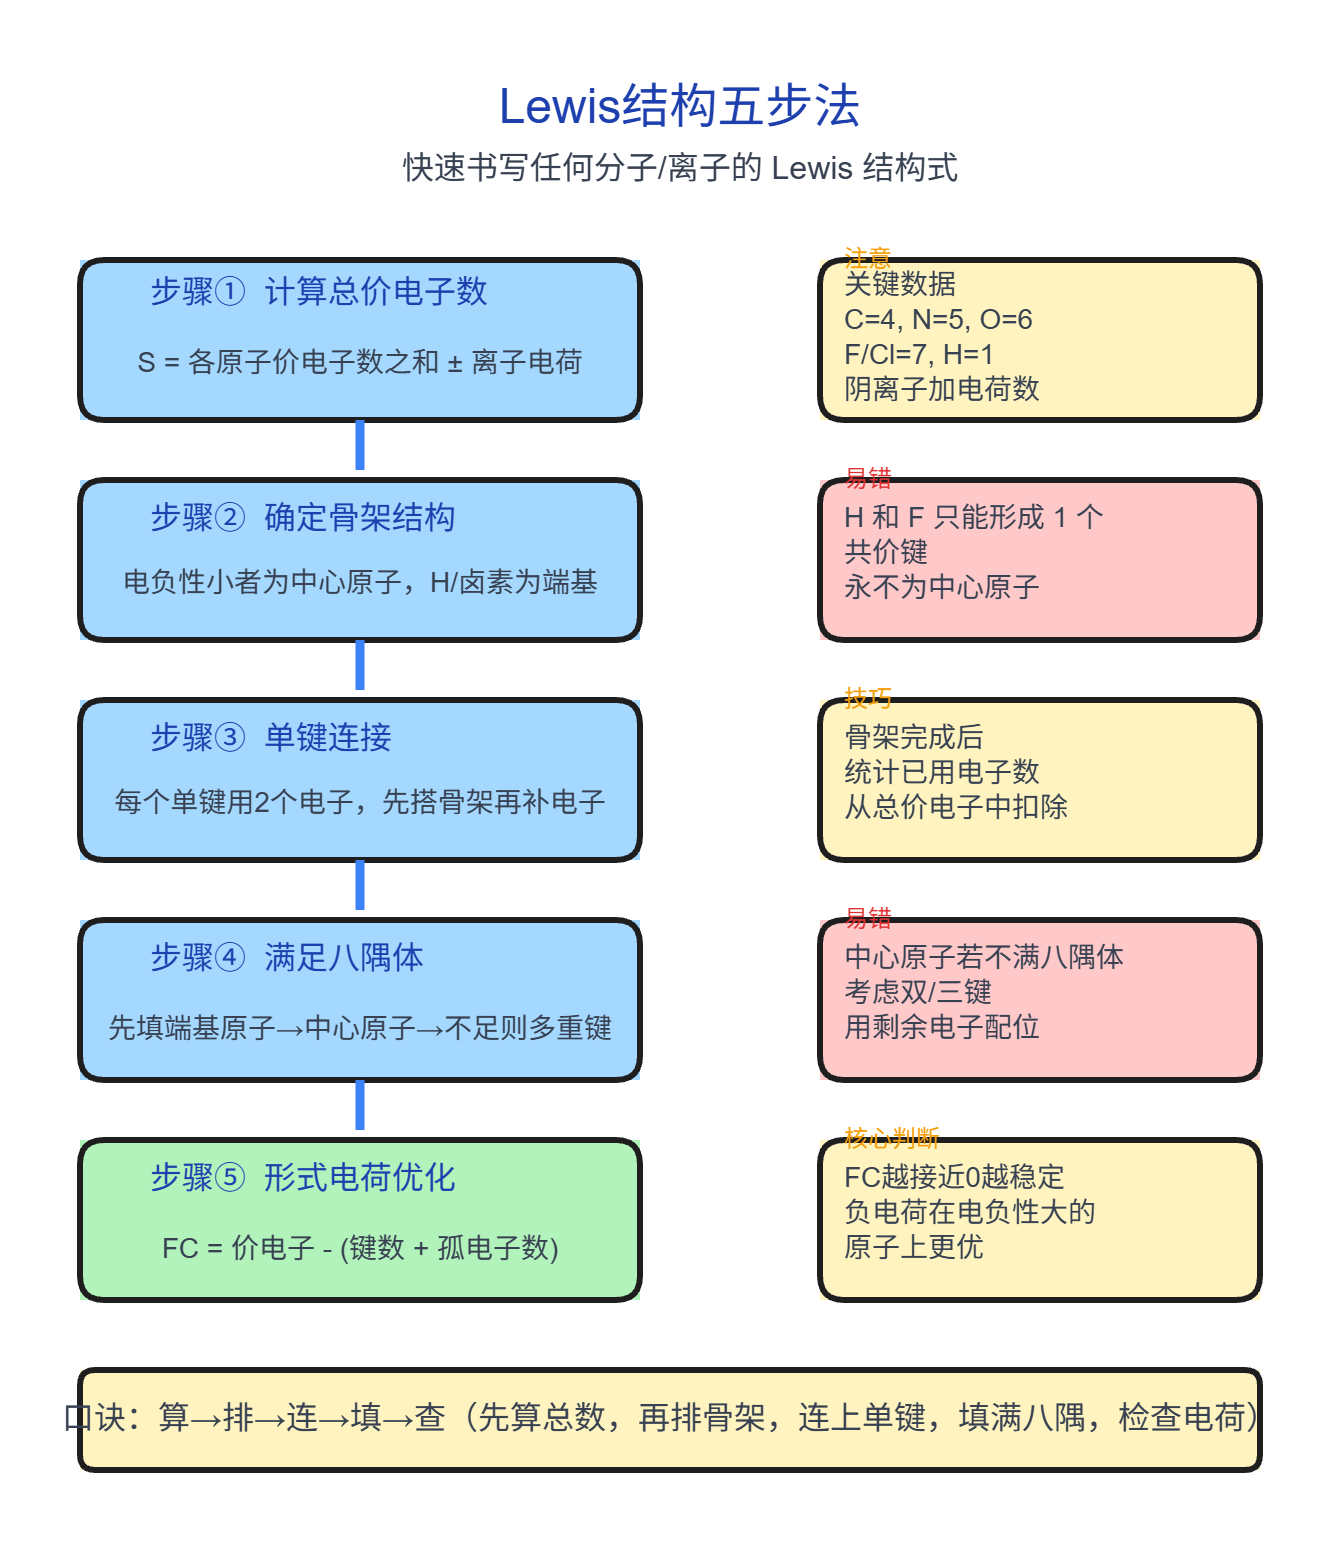
\includegraphics[width=0.9\textwidth,keepaspectratio]{media/Lewis五步法流程.流程图.png}
\caption{图 Lewis结构五步法流程图。左列五步流程，右列每步的关键提示与常见错误，底部口诀便于记忆。}
\end{figure}

\textbf{例}：NO\textsubscript{3}\textsuperscript{-} 的 Lewis 结构
- S = N(5) + O(6×3) + 1(负电荷) = 24 个价电子
- 骨架：N 居中，3 个 O 在端基
- 3 个 N-O 单键用去 6e\textsuperscript{-}，剩余 18e\textsuperscript{-} → 3 个 O 各分 6e\textsuperscript{-}（3 对孤对）
- N 只有 6e\textsuperscript{-} → 将一个 O 的 1 对孤对改为双键 → N 达到 8e\textsuperscript{-}

\begin{quote}
📝 \textbf{算一算}：按五步法完成以下分子的 Lewis 结构，先算总价电子数：
\textbar{} 分子/离子 \textbar{} 总价电子数 S \textbar{} 骨架 \textbar{} 中心是否满足八隅体？ \textbar{} 是否有孤对？ \textbar{}
\textbar:---:\textbar:---:\textbar:---\textbar:---:\textbar:---:\textbar{}
\textbar{} CO\textsubscript{2} \textbar{} 16 \textbar{} O-C-O \textbar{} ✅ \textbar{} 每个 O 有 2 对孤对 \textbar{}
\textbar{} SO\textsubscript{2} \textbar{} \_\_\_\_ \textbar{} \_\_\_\_ \textbar{} \_\_\_\_ \textbar{} \_\_\_\_ \textbar{}
\textbar{} ClO\textsubscript{4}\textsuperscript{-} \textbar{} \_\_\_\_ \textbar{} \_\_\_\_ \textbar{} \_\_\_\_ \textbar{} \_\_\_\_ \textbar{}
\textbar{} BrF\textsubscript{3} \textbar{} \_\_\_\_ \textbar{} \_\_\_\_ \textbar{} \_\_\_\_ \textbar{} \_\_\_\_ \textbar{}
（答案在 §十 参考答案）*
\end{quote}

\subsubsection{1.3 形式电荷（Formal Charge）}\label{ux5f62ux5f0fux7535ux8377formal-charge}

\[
\text{FC} = \text{价电子数} - \text{孤对电子数} - \frac{1}{2} \times \text{成键电子数}
\]

\textbf{最优结构选择原则}（按优先级）：
1. 形式电荷绝对值之和最小
2. 负电荷在电负性大的原子上
3. 避免同号电荷在相邻原子上

\begin{quote}
🧠 \textbf{教学洞察}：中文化学命名中的''形式电荷''常译作''形式电荷''，但这个''形式''二字正是最大的误导源------学生最容易犯的错误就是认为形式电荷就是该原子的实际电荷。\textbf{FC = -1 不意味着该原子带 1 个负电荷，它只是一个人为分配的''表观电荷''，用来在不同共振结构之间做比较的。} CO 分子中 C 的形式电荷为 -1、O 为 +1，但实验测得 CO 的偶极矩方向为 C\textsuperscript{-}→O\textsuperscript{+} 吗？非也------实际 CO 的偶极矩极小且方向是 C\textsuperscript{+}→O\textsuperscript{-}。这就证明形式电荷 ≠ 实际电荷。
\end{quote}

\begin{quote}
⚠️ \textbf{易错点}：形式电荷计算中，\textbf{孤对电子数和成键电子数要分清楚}。初学者常见错误是：将双键的 4 个电子全部计入''成键电子''，但公式中的''成键电子数''指的是与该原子直接相连的共价键中的总电子数------双键算 4 个。公式为 \(\text{FC} = \text{价电子数} - \text{孤对电子数} - \frac{1}{2} \times \text{成键电子数}\)。
\end{quote}

\subsubsection{1.4 共振结构}\label{ux5171ux632fux7ed3ux6784}

当单个 Lewis 结构无法准确描述电子分布时，需要多个 Lewis 结构共同描述------\textbf{共振杂化体}。

\textbf{书写要点}：
- 各共振式中原子位置固定（不是同分异构体）
- 各共振式中孤对电子数相等
- 形式电荷为 0 的结构最稳定

\textbf{例}：NO\textsubscript{3}\textsuperscript{-} 的三个等价共振结构：

\begin{figure}[H]\centering
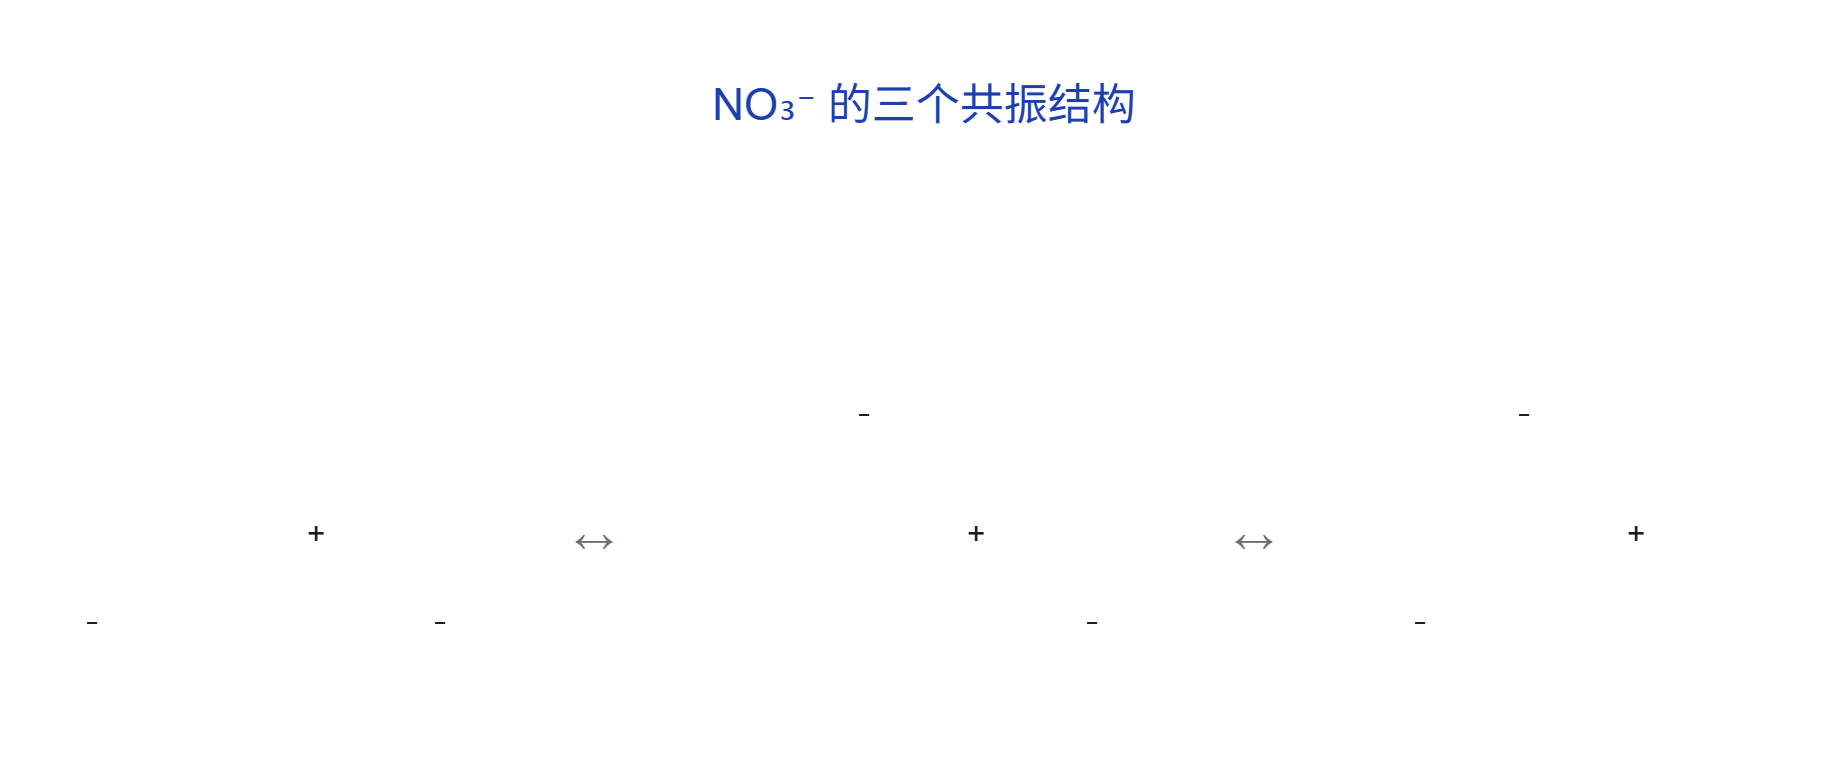
\includegraphics[width=0.9\textwidth,keepaspectratio]{media/NO3-共振结构.lewis.png}

\end{figure}

\emph{图 NO\textsubscript{3}\textsuperscript{-} 的三个等价共振结构（从左到右：双键分别在顶端、左下、右下三个位置）。各共振式中 N 的形式电荷均为 +1，单键连接的 O\textsuperscript{-} 为 -1，双键连接的 O 为 0。三个结构叠加得到 N-O 键平均键级为 1⅓。}

实际 N-O 键长均等（介于单键和双键之间），说明电子离域到整个 NO\textsubscript{3}\textsuperscript{-} 离子中。

相关 KP：Lewis结构式

\begin{center}\rule{0.5\linewidth}{0.5pt}\end{center}

\subsection{二、VSEPR 理论 ------ 猜形状}\label{ux4e8cvsepr-ux7406ux8bba-ux731cux5f62ux72b6}

为什么 Lewis 结构还不够？因为知道电子怎么连只是第一步------我们还需要知道分子在\textbf{三维空间里长什么样}。NH\textsubscript{3} 是平面三角形还是三角锥形？这决定了它有没有极性（NH\textsubscript{3} 是极性分子，BF\textsubscript{3} 是非极性）。

VSEPR 理论的价值就在于此：\textbf{从 Lewis 结构中的电子对数目，推断分子的三维形状。} 它不考虑复杂的量子力学，只用''电子对互相排斥''这一条直觉，就能准确预测绝大多数分子的构型------包括很多''反直觉''的情况（比如 XeF\textsubscript{2} 明明是三个原子却是直线形）。

\begin{quote}
💡 \textbf{关键定位}：VSEPR 是''描述性''理论------它告诉我们\textbf{是什么形状}，但不告诉我们\textbf{为什么是这个形状}。后面的杂化轨道理论才回答''为什么''。
\end{quote}

\begin{figure}[H]\centering
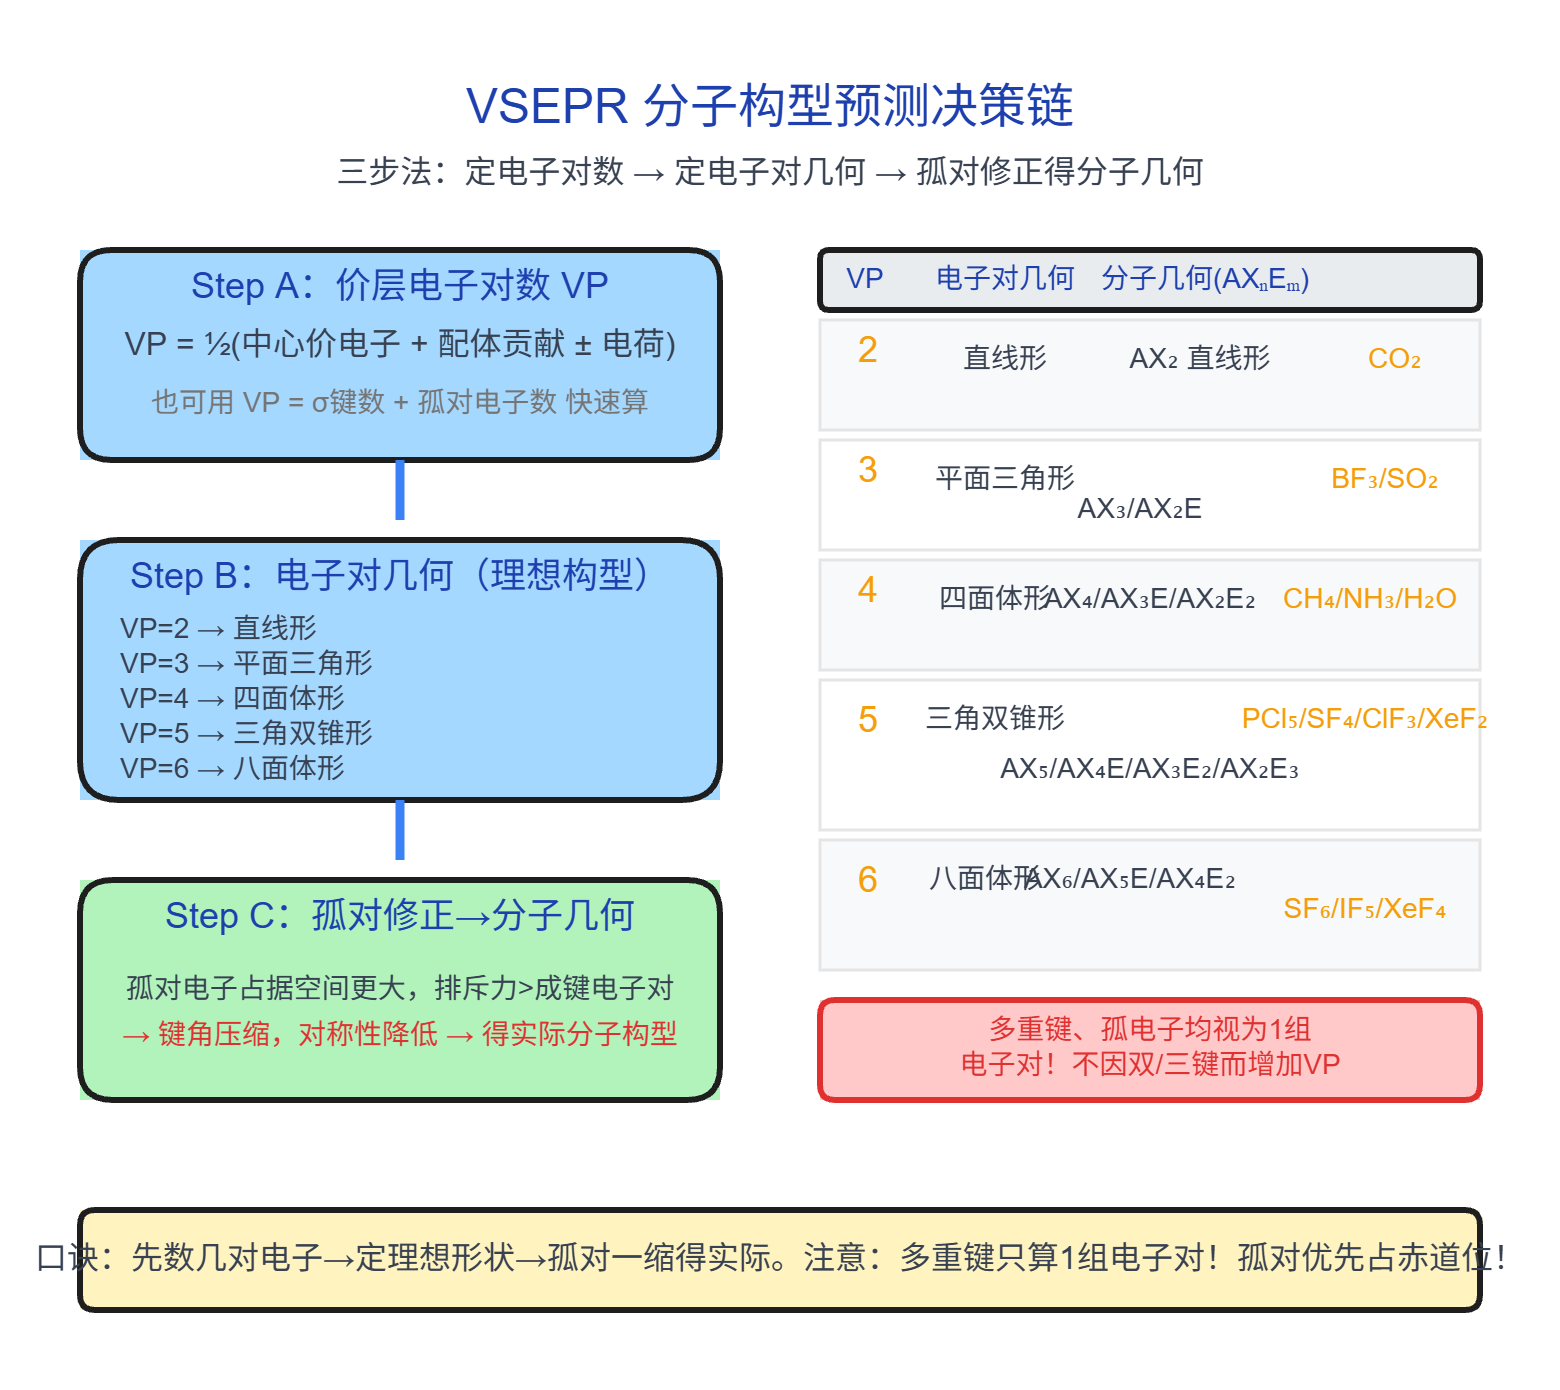
\includegraphics[width=0.9\textwidth,keepaspectratio]{media/VSEPR决策链.流程图.png}
\caption{图 VSEPR 决策链流程图。左侧为三步决策流程（Step A→B→C），右侧为 AXₙEₘ 完整构型速查表（VP=2 至 VP=6），底部口诀便于记忆。注意：多重键只算 1 组电子对！}
\end{figure}

\subsubsection{2.1 核心思想}\label{ux6838ux5fc3ux601dux60f3}

\textbf{价层电子对互斥理论}：价层电子对（成键电子对 + 孤对电子）互相排斥，趋向于尽可能远离。

\subsubsection{2.2 AXₙEₘ 模型}\label{axux2099eux2098-ux6a21ux578b}

\begin{itemize}
\tightlist
\item
  A = 中心原子
\item
  X = 配位原子（成键电子对）
\item
  E = 孤对电子
\item
  n + m = 价层电子对总数
\end{itemize}

{\def\LTcaptype{none} % do not increment counter
\begin{longtable}[]{@{}clllcl@{}}
\toprule\noalign{}
总电子对数 & 理想排布 & 分子类型 & 实际构型 & 键角 & 实例 \\
\midrule\noalign{}
\endhead
\bottomrule\noalign{}
\endlastfoot
2 & 直线形 & AX\textsubscript{2} & 直线形 & 180° & BeCl\textsubscript{2}、CO\textsubscript{2} \\
3 & 平面三角形 & AX\textsubscript{3} & 平面三角形 & 120° & BF\textsubscript{3}、NO\textsubscript{3}\textsuperscript{-} \\
& & AX\textsubscript{2}E & V 形 & \textless120° & SO\textsubscript{2}、O\textsubscript{3} \\
4 & 四面体 & AX\textsubscript{4} & 四面体 & 109.5° & CH\textsubscript{4}、NH\textsubscript{4}\textsuperscript{+} \\
& & AX\textsubscript{3}E & 三角锥形 & \textless109.5° & NH\textsubscript{3}(107°) \\
& & AX\textsubscript{2}E\textsubscript{2} & V 形 & \textless109.5° & H\textsubscript{2}O(104.5°) \\
5 & 三角双锥 & AX\textsubscript{5} & 三角双锥 & 90°/120° & PCl\textsubscript{5} \\
& & AX\textsubscript{4}E & 跷跷板形 & --- & SF\textsubscript{4} \\
& & AX\textsubscript{3}E\textsubscript{2} & T 形 & --- & ClF\textsubscript{3} \\
& & AX\textsubscript{2}E\textsubscript{3} & 直线形 & --- & XeF\textsubscript{2} \\
6 & 八面体 & AX\textsubscript{6} & 八面体 & 90° & SF\textsubscript{6} \\
& & AX\textsubscript{5}E & 四方锥形 & --- & BrF\textsubscript{5} \\
& & AX\textsubscript{4}E\textsubscript{2} & 平面正方形 & --- & XeF\textsubscript{4} \\
\end{longtable}
}

\begin{figure}[H]\centering
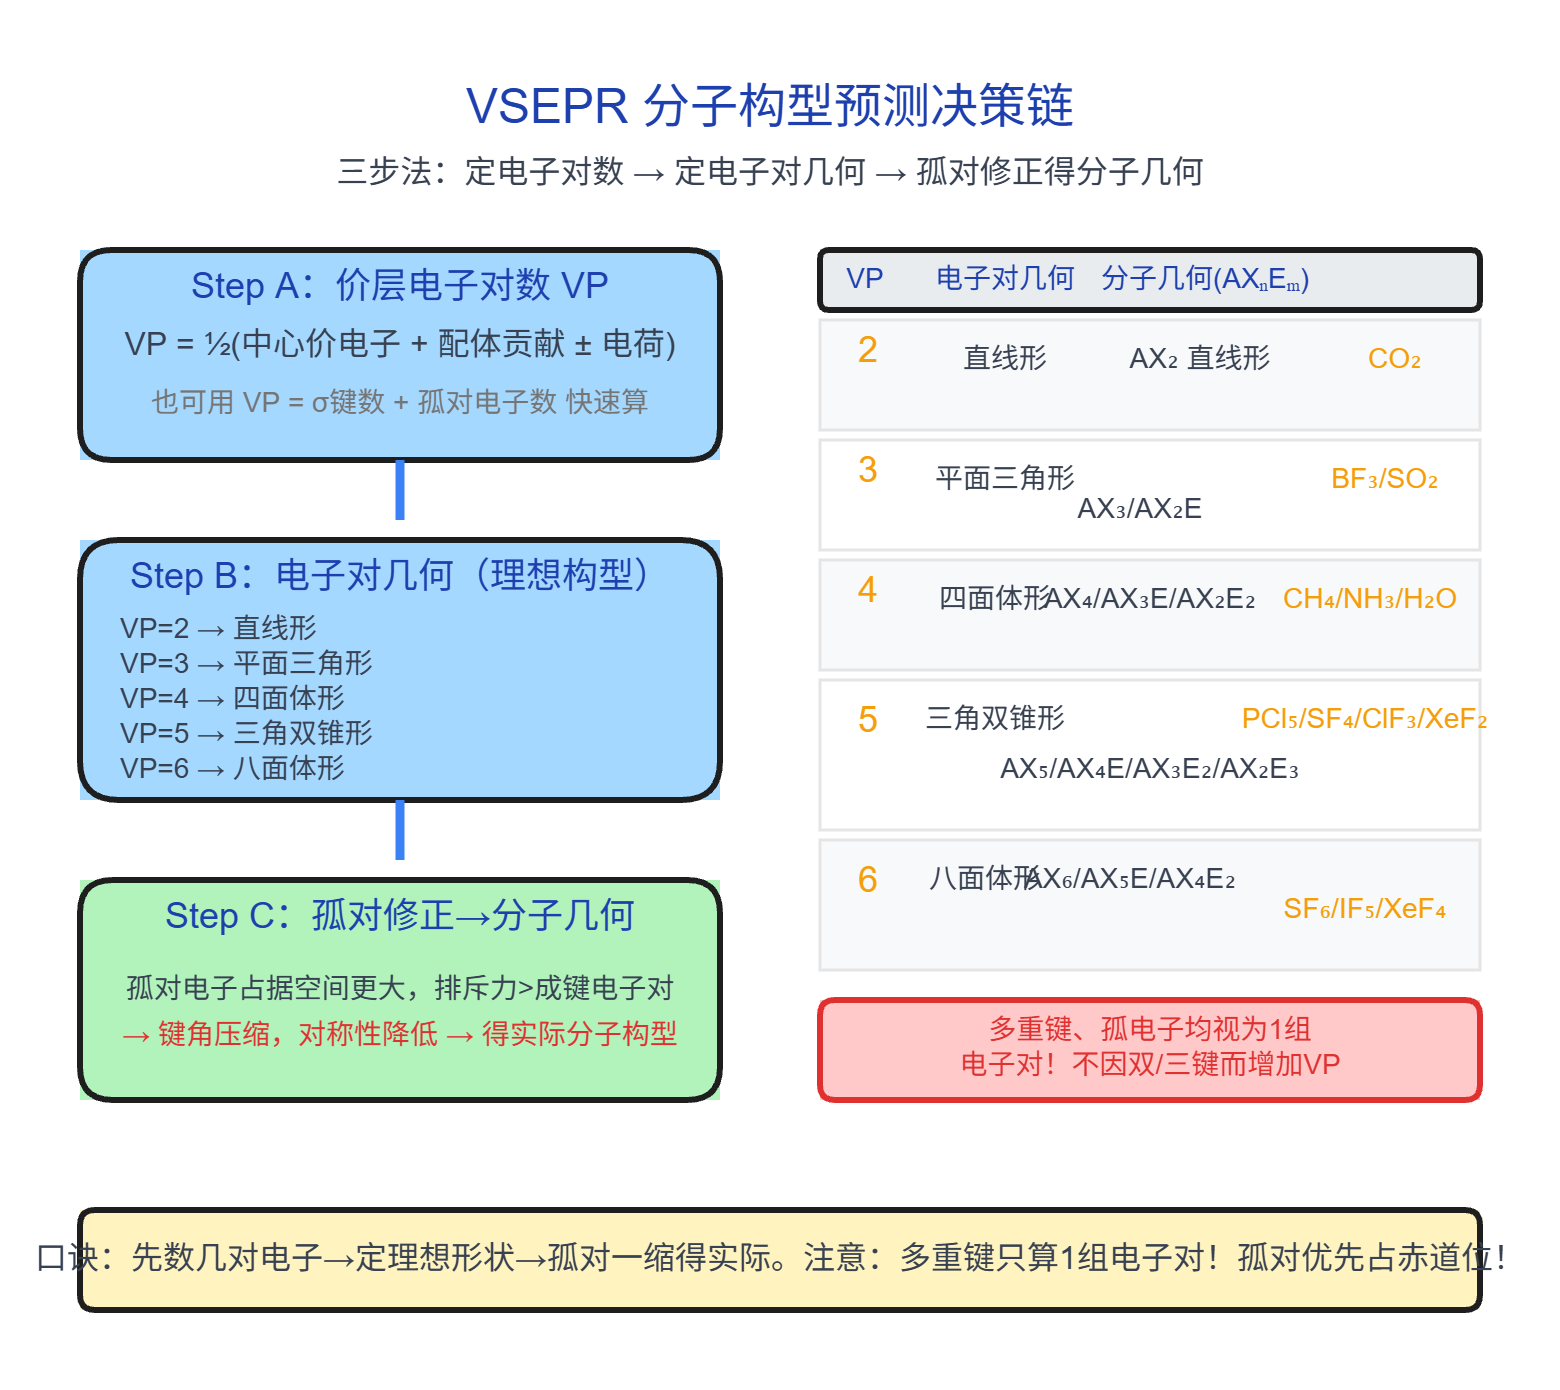
\includegraphics[width=0.9\textwidth,keepaspectratio]{media/VSEPR决策链.流程图.png}
\caption{图 VSEPR 分子构型汇总 — 从 AX2 到 AX6 的理想几何与孤对电子修正构型（上：AXₙ 型；中：AX4 衍生；下：AX5/AX6 衍生）}
\end{figure}

\begin{quote}
📝 \textbf{练一练}：根据 VSEPR 模型填写下表（答案在 §十）：
\textbar{} 分子 \textbar{} 总电子对数 \textbar{} 成键数 n \textbar{} 孤对数 m \textbar{} AXₙEₘ \textbar{} 理想排布 \textbar{} 实际构型 \textbar{}
\textbar:---:\textbar:---:\textbar:---:\textbar:---:\textbar:---:\textbar:---\textbar:---\textbar{}
\textbar{} SF\textsubscript{4} \textbar{} 5 \textbar{} 4 \textbar{} 1 \textbar{} AX\textsubscript{4}E \textbar{} 三角双锥 \textbar{} 跷跷板形 \textbar{}
\textbar{} ClF\textsubscript{3} \textbar{} \_\_\_\_ \textbar{} \_\_\_\_ \textbar{} \_\_\_\_ \textbar{} \_\_\_\_ \textbar{} \_\_\_\_ \textbar{} \_\_\_\_ \textbar{}
\textbar{} XeF\textsubscript{2} \textbar{} \_\_\_\_ \textbar{} \_\_\_\_ \textbar{} \_\_\_\_ \textbar{} \_\_\_\_ \textbar{} \_\_\_\_ \textbar{} \_\_\_\_ \textbar{}
\textbar{} IF\textsubscript{4}\textsuperscript{-} \textbar{} \_\_\_\_ \textbar{} \_\_\_\_ \textbar{} \_\_\_\_ \textbar{} \_\_\_\_ \textbar{} \_\_\_\_ \textbar{} \_\_\_\_ \textbar{}
\emph{提示：先算中心原子的价层电子总数（考虑配体贡献和离子电荷），÷2 得电子对数，再减去成键数得孤对数。}
\end{quote}

\subsubsection{2.3 关键规则}\label{ux5173ux952eux89c4ux5219}

\textbf{孤对电子的位置选择}：
- 在三角双锥体系（5 对电子）中，孤对电子\textbf{优先占据赤道向位置}（夹角 120°，空间更大），而非轴向位置（夹角 90°，排斥更强）。
- 记忆口诀：\textbf{``孤对先占赤道位，90° 最少为赢''}
- 类比：\textbf{``大胖子（孤对电子）坐赤道位，旁边只要忍受 2 个 90° 的人；坐轴向位要忍 3 个。''}

\begin{quote}
🧠 \textbf{教学洞察}：孤对电子的位置选择是最容易被忽视的高频考点。SF\textsubscript{4}（AX\textsubscript{4}E，跷跷板形）中孤对放赤道位、ClF\textsubscript{3}（AX\textsubscript{3}E\textsubscript{2}，T 形）中两对孤对都放赤道位------记忆核心不是背形状，而是理解''最小化 90° 排斥''原则。对于 5 对电子的三角双锥体系，\textbf{孤对优先占赤道 → 赤道位留给孤对 → 轴向位留给配体}。
\end{quote}

\textbf{排斥力大小顺序}：
\[
\text{孤对–孤对} > \text{孤对–成键} > \text{成键–成键}
\]

\begin{quote}
⚠️ \textbf{易错点}：NH\textsubscript{3} 的键角为什么是 107° 而非 109.5°？因为 1 对孤对的排斥 \textgreater{} 1 个成键对的排斥 → 孤对压缩 H-N-H 键角。H\textsubscript{2}O 更狠------2 对孤对！压缩到 104.5°。\textbf{每多 1 对孤对，键角被压缩约 2°--2.5°}（粗略估算，但有用）。
\end{quote}

\textbf{多重键的处理}：多重键视为 \textbf{1 个电子对区域}。例如 CO\textsubscript{2} 中 C 与 O 各形成一个双键，共 2 个电子对区域 → 直线形。

\begin{quote}
💡 \textbf{常见误解}：双键有 4 个电子，三键有 6 个电子------为什么在 VSEPR 中都只算 1 个区域？因为这些电子都在\textbf{同一方向}（都在键轴上或都在垂直于键轴的方向上），它们的排斥效应等价于 1 组电子对。记忆：\textbf{``多重键的电子对都在同一方向怼你，算 1 组就够了。''}
\end{quote}

相关 KP：VSEPR理论

\begin{center}\rule{0.5\linewidth}{0.5pt}\end{center}

\subsection{三、杂化轨道理论 ------ 解释为什么}\label{ux4e09ux6742ux5316ux8f68ux9053ux7406ux8bba-ux89e3ux91caux4e3aux4ec0ux4e48}

VSEPR 告诉我们分子''长什么样''，但没告诉我们\textbf{为什么}。为什么 CH\textsubscript{4} 是正四面体而不是平面正方形？为什么 H\textsubscript{2}O 的键角不是 90°（如果只用纯 p 轨道成键）而是 104.5°？

答案是：\textbf{电子轨道的''混合''}------杂化。

\begin{quote}
💡 \textbf{关键定位}：VSEPR 是''描述性''理论（告诉我们是什么形状），杂化轨道理论是''解释性''理论（告诉我们为什么是那个形状）。两者互相配合：先 VSEPR 预测形状，再杂化解释形状。\textbf{千万不要反过来}------不要从杂化类型推构型，而要从构型反推杂化类型。
\end{quote}

\textbf{核心思想}：中心原子的能量相近的原子轨道（ns + np + nd）在成键过程中\textbf{线性组合}成数量相等、能量相同的\textbf{杂化轨道}，用于与配位原子成键。

\begin{quote}
🧠 \textbf{教学洞察}：学生最容易犯的概念性错误是把杂化当作原子的''固有属性''------他们问''CH\textsubscript{4} 中的 C 是什么杂化？``仿佛 C 原子天生就是 sp\textsuperscript{3} 杂化。\textbf{但杂化发生在成键过程中，不是原子固有的。} 孤立 C 原子的基态是 2s\textsuperscript{2}2p\textsuperscript{2}，只有在形成 4 个 C-H 键时，1 个 2s 电子被激发到 2p 空轨道，然后 1 个 2s + 3 个 2p 轨道杂化成 4 个 sp\textsuperscript{3} 杂化轨道------这是成键的''后果''，不是''前提''。
类比：\textbf{``混色------红色（s 轨道）+ 蓝色（p 轨道）→ 紫色（sp 杂化轨道）。紫色既不是红也不是蓝，但包含了红和蓝的成分。而混合只是在你需要画画（成键）的时候才发生，不是颜料本身一直是混合的。''}
\end{quote}

\subsubsection{3.1 杂化类型与几何构型}\label{ux6742ux5316ux7c7bux578bux4e0eux51e0ux4f55ux6784ux578b}

{\def\LTcaptype{none} % do not increment counter
\begin{longtable}[]{@{}clclcl@{}}
\toprule\noalign{}
杂化类型 & 参与轨道 & 杂化轨道数 & 空间构型 & 键角 & 实例 \\
\midrule\noalign{}
\endhead
\bottomrule\noalign{}
\endlastfoot
sp & s + p & 2 & 直线形 & 180° & BeCl\textsubscript{2}、CO\textsubscript{2} \\
sp\textsuperscript{2} & s + p + p & 3 & 平面三角形 & 120° & BF\textsubscript{3}、NO\textsubscript{3}\textsuperscript{-}、石墨 \\
sp\textsuperscript{3} & s + p + p + p & 4 & 四面体 & 109.5° & CH\textsubscript{4}、NH\textsubscript{3}、H\textsubscript{2}O \\
sp\textsuperscript{3}d & s + p + p + p + d & 5 & 三角双锥 & 90°/120° & PCl\textsubscript{5} \\
sp\textsuperscript{3}d\textsuperscript{2} & s + p + p + p + d + d & 6 & 八面体 & 90° & SF\textsubscript{6} \\
\end{longtable}
}

\begin{figure}[H]\centering
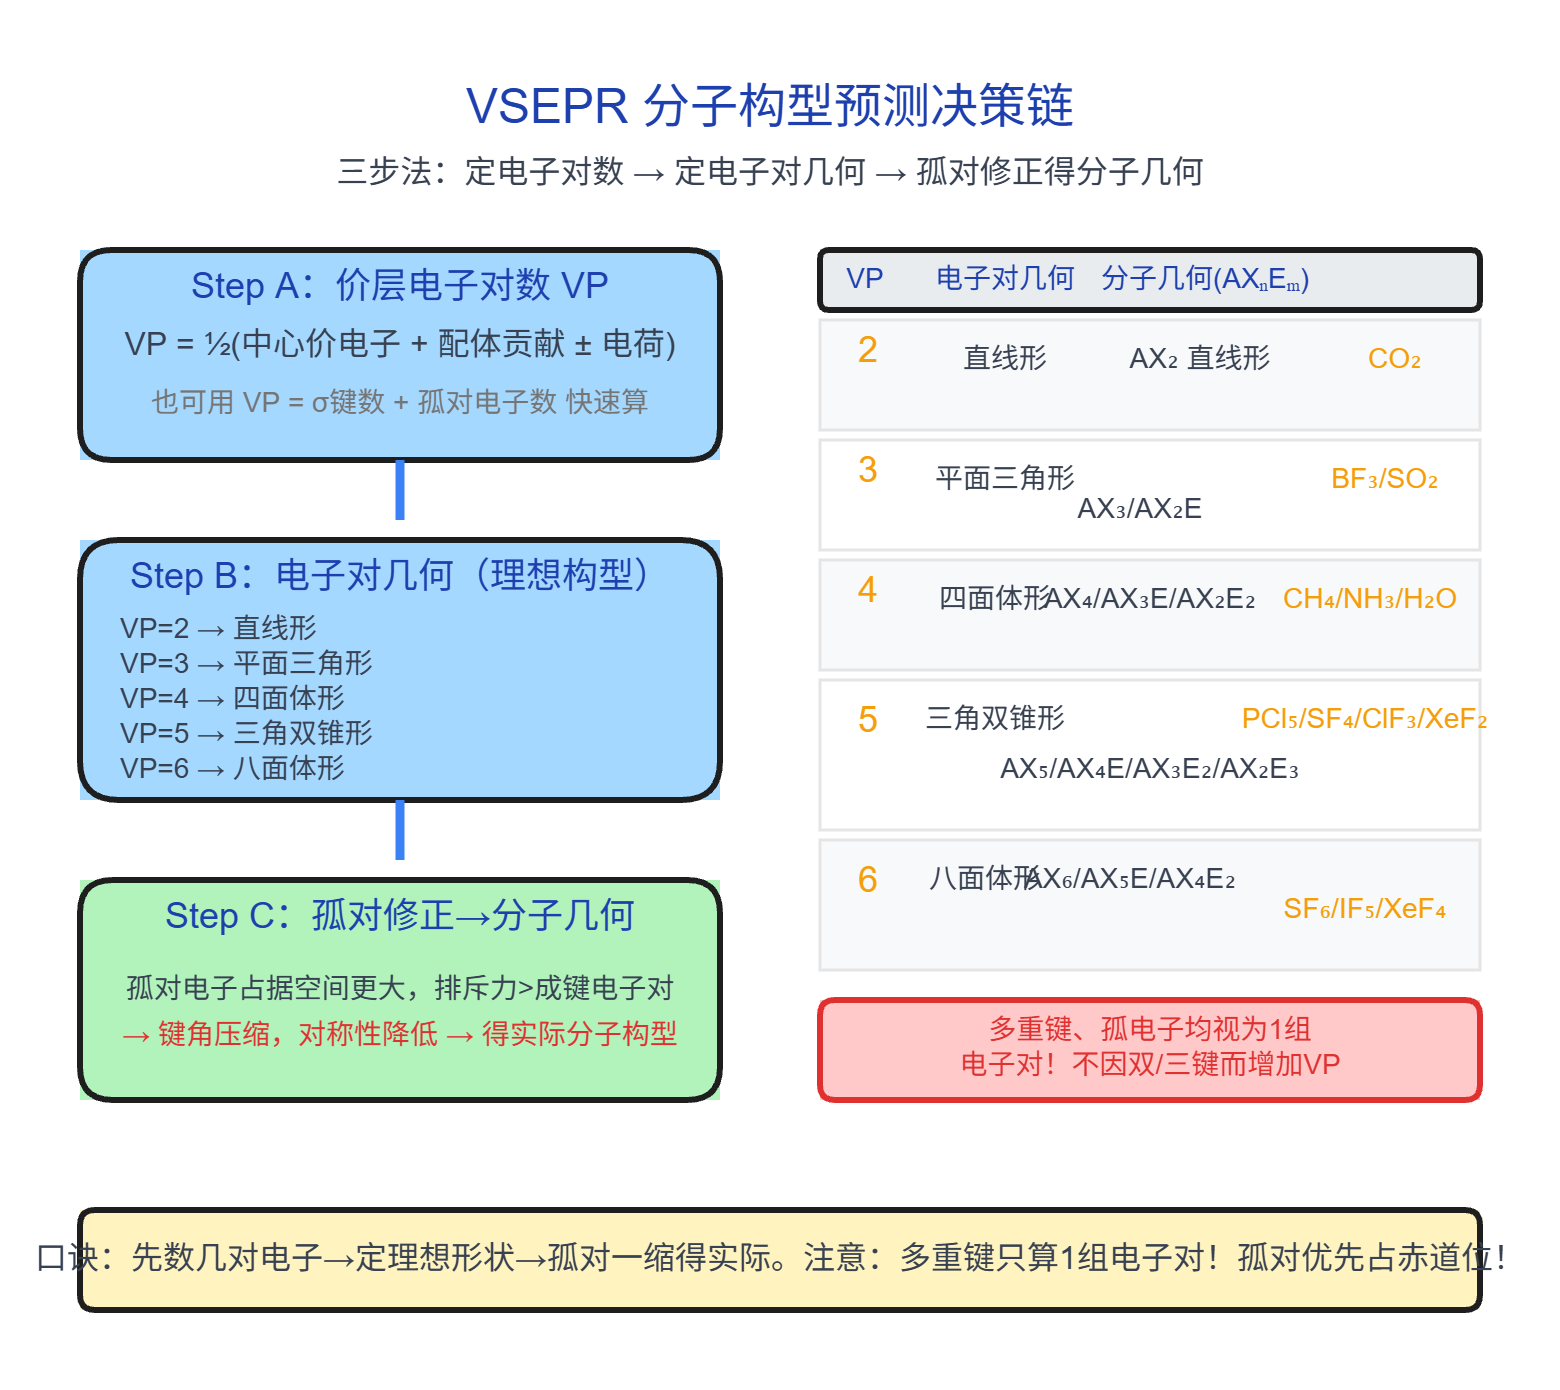
\includegraphics[width=0.9\textwidth,keepaspectratio]{media/VSEPR决策链.流程图.png}
\caption{图 常见杂化构型 — CH4（sp3 四面体，左）、BCl3（sp2 平面三角形，中）、BeCl2（sp 直线形，右）}
\end{figure}

\begin{figure}[H]\centering
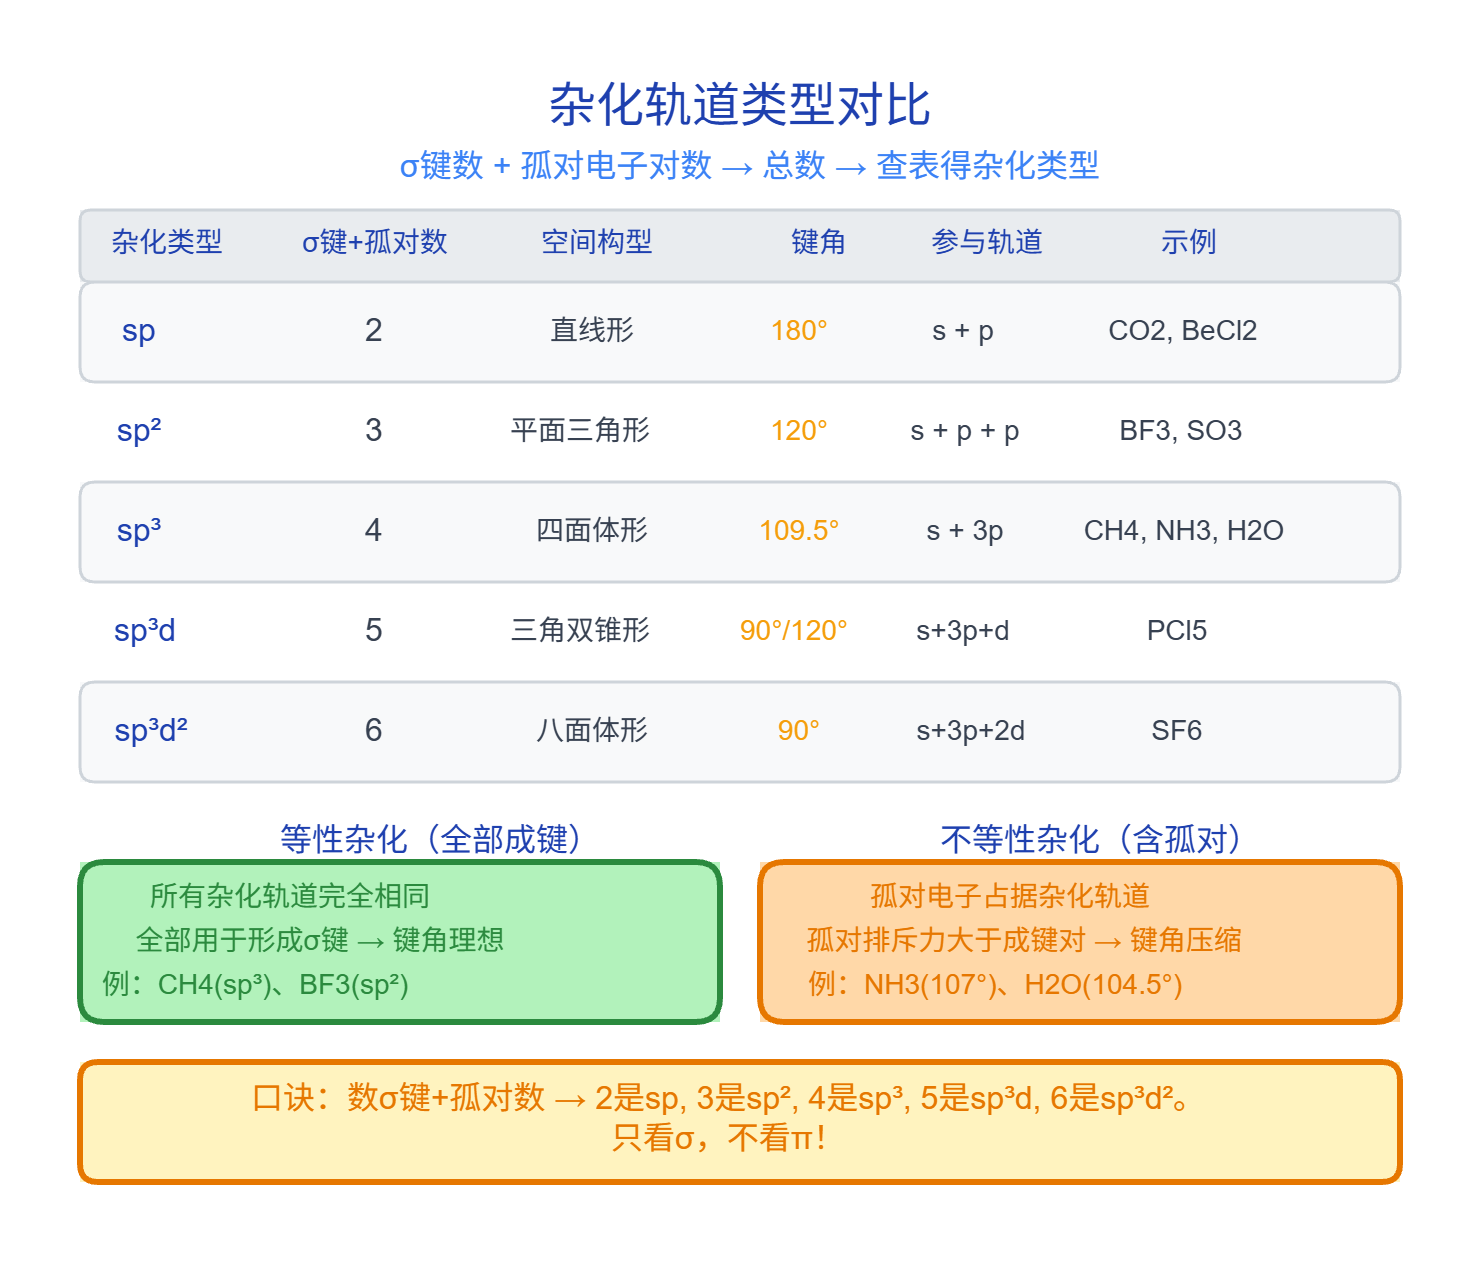
\includegraphics[width=0.9\textwidth,keepaspectratio]{media/轨道杂化类型对比.关系图.png}
\caption{图 杂化轨道类型对比。左列五类杂化（sp/sp2/sp3/sp3d/sp3d2）参数对比，右下侧等性/不等性杂化辨析，底部口诀便于记忆。}
\end{figure}

\subsubsection{3.2 等性杂化 vs 不等性杂化}\label{ux7b49ux6027ux6742ux5316-vs-ux4e0dux7b49ux6027ux6742ux5316}

{\def\LTcaptype{none} % do not increment counter
\begin{longtable}[]{@{}
  >{\raggedright\arraybackslash}p{(\linewidth - 8\tabcolsep) * \real{0.1905}}
  >{\raggedright\arraybackslash}p{(\linewidth - 8\tabcolsep) * \real{0.1905}}
  >{\raggedright\arraybackslash}p{(\linewidth - 8\tabcolsep) * \real{0.1905}}
  >{\centering\arraybackslash}p{(\linewidth - 8\tabcolsep) * \real{0.2381}}
  >{\raggedright\arraybackslash}p{(\linewidth - 8\tabcolsep) * \real{0.1905}}@{}}
\toprule\noalign{}
\begin{minipage}[b]{\linewidth}\raggedright
类型
\end{minipage} & \begin{minipage}[b]{\linewidth}\raggedright
特征
\end{minipage} & \begin{minipage}[b]{\linewidth}\raggedright
s/p 成分分布
\end{minipage} & \begin{minipage}[b]{\linewidth}\centering
键角
\end{minipage} & \begin{minipage}[b]{\linewidth}\raggedright
实例
\end{minipage} \\
\midrule\noalign{}
\endhead
\bottomrule\noalign{}
\endlastfoot
\textbf{等性杂化} & 所有杂化轨道含相同的 s/p 成分 & 各轨道 s\% 相同 & 相等（理想键角） & CH\textsubscript{4}（109.5°）、BF\textsubscript{3}（120°） \\
\textbf{不等性杂化} & 孤对电子占据的杂化轨道 s 成分较高 & 孤对轨道 s\% \textgreater{} 成键轨道 s\% & 被压缩 & NH\textsubscript{3}（107°）、H\textsubscript{2}O（104.5°） \\
\end{longtable}
}

\begin{quote}
🧠 \textbf{教学洞察}：不等性杂化的本质是\textbf{孤对电子占据的杂化轨道 s 成分更高}。因为 s 轨道能量比 p 轨道低，孤对电子''想要''能量更低的轨道。结果就是: 孤对占据的杂化轨道含更多 s 成分（能量更低），而成键轨道含更多 p 成分（能量更高）→ 键角被压缩。这就是为什么 NH\textsubscript{3}（1 对孤对，压缩至 107°）的键角大于 H\textsubscript{2}O（2 对孤对，压缩至 104.5°）------孤对越多，压缩越厉害！
\end{quote}

\begin{quote}
🧠 \textbf{教学洞察}：等性/不等性杂化的快速判断 ------ 中心原子参与杂化的轨道中，只要\textbf{有已成对的电子}参与杂化，通常就是不等性杂化。或者说：\textbf{m = n（电子对数 = 配体数）→ 等性；m \textgreater{} n（有孤对）→ 不等性}。
\end{quote}

\subsubsection{3.3 操作口诀}\label{ux64cdux4f5cux53e3ux8bc0}

\textbf{``sp 看 σ 键+孤对电子数：2→sp, 3→sp\textsuperscript{2}, 4→sp\textsuperscript{3}''}
\textbf{``只看 σ，不看 π''}
\textbf{``等性杂化键全同，不等性杂化有孤对''}

\begin{quote}
⚠️ \textbf{易错点}：杂化判断的两个最常犯错误------(1) \textbf{用 VSEPR 构型直接反推杂化}，认为直线型一定 sp（忽略了 XeF\textsubscript{2} 直线形但是 sp\textsuperscript{3}d）、三角双锥一定 sp\textsuperscript{3}d（忽略了是否真用到 d 轨道）；(2) \textbf{看到碳就认为是 sp\textsuperscript{3}}------碳有双键时是 sp\textsuperscript{2}（如 C\textsubscript{2}H\textsubscript{4}），有三键时是 sp（如 C\textsubscript{2}H\textsubscript{2}）。正确方法是：\textbf{数 σ 键数 + 孤对电子对数 → 总和 → 查表}。
\end{quote}

\begin{quote}
💡 \textbf{快速判断法}：杂化方式 = σ 键数 + 孤对电子对数。只看 σ、不看 π（π 键不占杂化轨道）！
\end{quote}

\begin{quote}
📝 \textbf{练一练}：判断以下分子/离子的中心原子杂化类型：
\textbar{} 分子 \textbar{} VSEPR 构型 \textbar{} σ 键数 \textbar{} 孤对电子对数 \textbar{} 总数 \textbar{} 杂化类型 \textbar{}
\textbar:---\textbar:---\textbar:---:\textbar:---:\textbar:---:\textbar:---:\textbar{}
\textbar{} CO\textsubscript{2} \textbar{} 直线形 \textbar{} 2 \textbar{} 0 \textbar{} 2 \textbar{} sp \textbar{}
\textbar{} BF\textsubscript{3} \textbar{} 平面三角形 \textbar{} \_\_\_\_ \textbar{} \_\_\_\_ \textbar{} \_\_\_\_ \textbar{} \_\_\_\_ \textbar{}
\textbar{} H\textsubscript{2}O \textbar{} V 形 \textbar{} \_\_\_\_ \textbar{} \_\_\_\_ \textbar{} \_\_\_\_ \textbar{} \_\_\_\_ \textbar{}
\textbar{} SF\textsubscript{6} \textbar{} 八面体 \textbar{} \_\_\_\_ \textbar{} \_\_\_\_ \textbar{} \_\_\_\_ \textbar{} \_\_\_\_ \textbar{}
\textbar{} PCl\textsubscript{5} \textbar{} 三角双锥 \textbar{} \_\_\_\_ \textbar{} \_\_\_\_ \textbar{} \_\_\_\_ \textbar{} \_\_\_\_ \textbar{}
\textbar{} XeF\textsubscript{2} \textbar{} 直线形 \textbar{} \_\_\_\_ \textbar{} \_\_\_\_ \textbar{} \_\_\_\_ \textbar{} \_\_\_\_ \textbar{}
\emph{提示：XeF\textsubscript{2} 是直线形但杂化不是 sp------它在第三周期，用到了 d 轨道。}
\end{quote}

相关 KP：杂化轨道理论

\begin{center}\rule{0.5\linewidth}{0.5pt}\end{center}

\subsection{四、离域π键 ------ 超越定域键}\label{ux56dbux79bbux57dfux3c0ux952e-ux8d85ux8d8aux5b9aux57dfux952e}

学完 Lewis 结构和杂化轨道，你可能觉得''分子结构就这么回事了''------每个键就是一根线，要么单键要么双键。但事实并非如此简单。NO\textsubscript{3}\textsuperscript{-} 的三个 N-O 键为什么完全相等？1,3-丁二烯中间的 C-C 单键为什么比乙烷的 C-C 单键短？苯的六个 C-C 键为什么完全一样？

答案在于：\textbf{电子并不总是被''定域''在两个原子之间------它们可以在多个原子上''离域''}。这就是离域π键（也称大π键、共轭π键）。

\begin{quote}
💡 \textbf{竞赛风向标}：离域π键是初赛结构化学的高频考点（每年约 1-2 题），也是理解有机化学共轭体系的基础。判断 πₙᵐ 的关键在于\textbf{三条件缺一不可}------很多学生只记''平面 + 平行 p 轨道''，忘了检查 m \textless{} 2n。
\end{quote}

\subsubsection{4.1 形成条件}\label{ux5f62ux6210ux6761ux4ef6}

离域π键（大π键，πₙᵐ）是指电子在\textbf{三个或以上}原子的平行 p 轨道上离域形成的 π 键。

\textbf{形成条件}（缺一不可）：
1. ✅ \textbf{共面性}：所有参与原子在同一平面内
2. ✅ \textbf{平行 p 轨道}：各原子有未参与杂化的平行 p 轨道
3. ✅ \textbf{电子数 m \textless{} 2n}：离域电子数小于 p 轨道数的 2 倍（否则会形成满带）

\begin{figure}[H]\centering
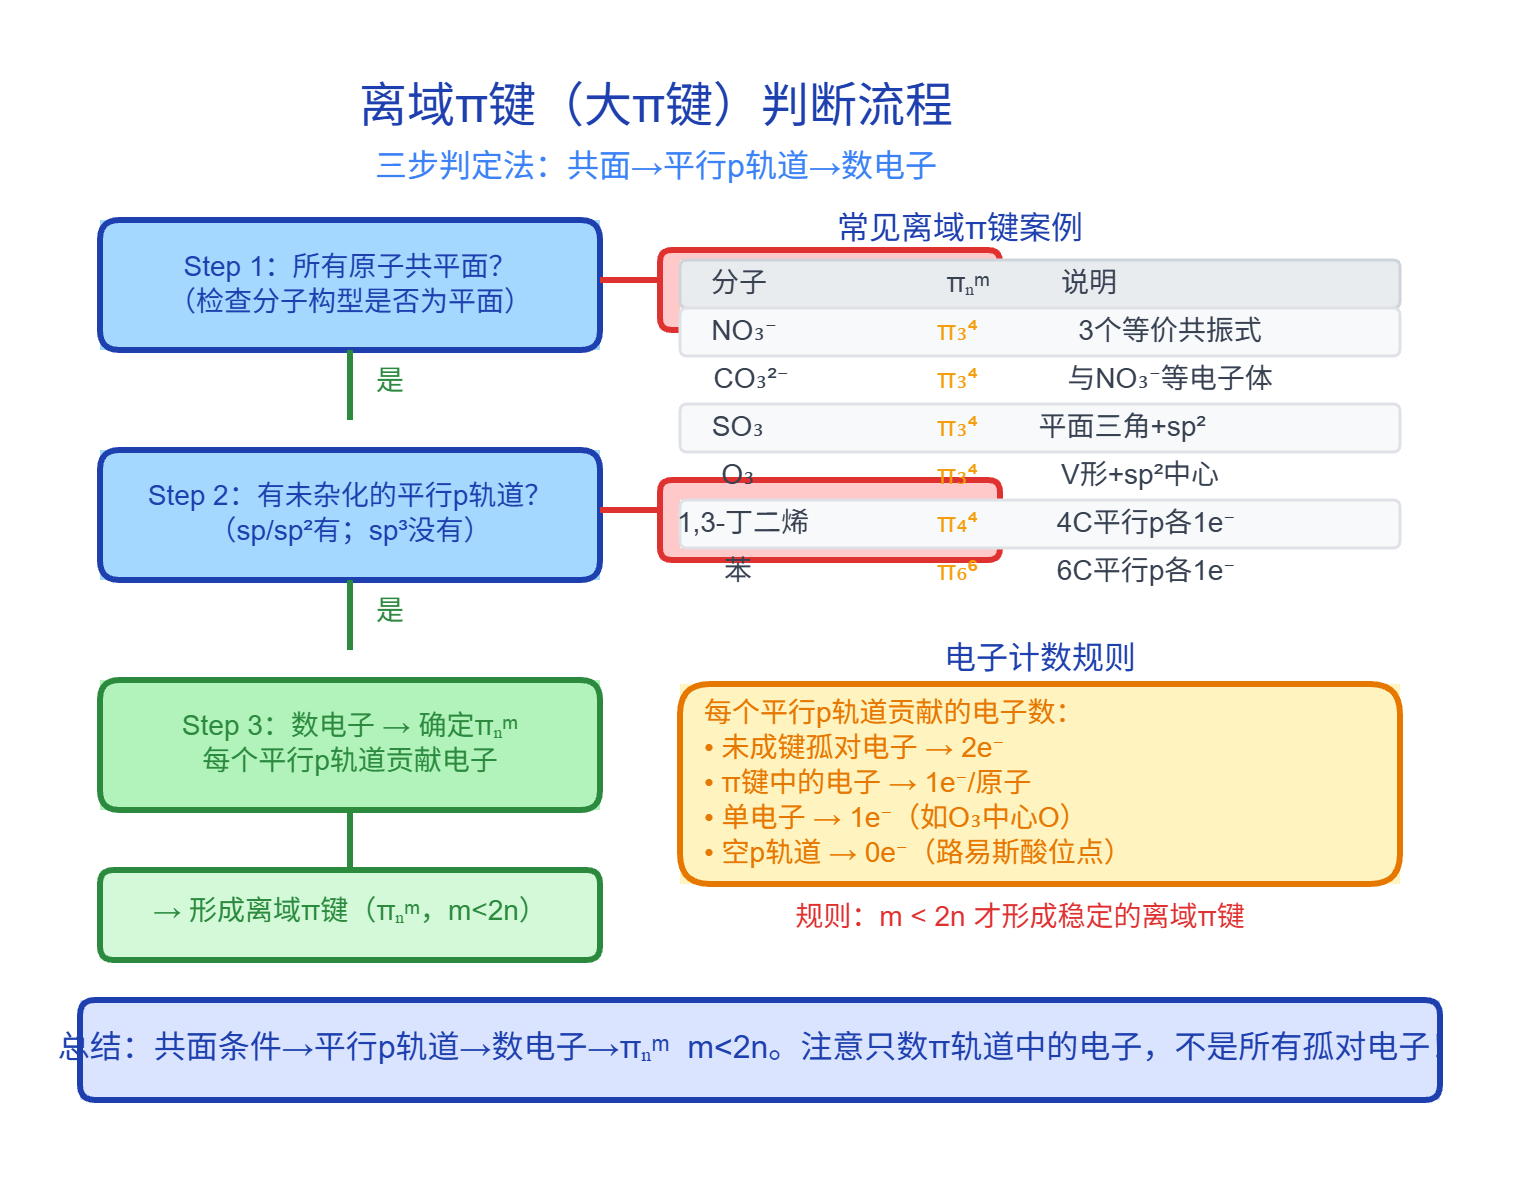
\includegraphics[width=0.9\textwidth,keepaspectratio]{media/离域π键判断流程.流程图.png}
\caption{图 离域π键判断流程。左侧三步决策链（共面→平行p轨道→数电子），右侧常见案例速查表（NO3-/CO32-/SO3/O3/丁二烯/苯）和电子计数规则。}
\end{figure}

\subsubsection{4.2 πₙᵐ 表示法}\label{ux3c0ux2099ux1d50-ux8868ux793aux6cd5}

\[
\pi_n^m
\]

\begin{itemize}
\tightlist
\item
  n = 参与离域的原子数（平行 p 轨道数）
\item
  m = 参与离域的电子数
\end{itemize}

\textbf{电子计数方法}：
1. 每个参与离域的原子提供 1 个 p 电子（若该原子在杂化后 p 轨道上有 1 个单电子）
2. 若 p 轨道为空的（如缺电子体系），提供 0 个电子
3. 若 p 轨道有 2 个电子（如孤对电子在 p 轨道上），提供 2 个电子
4. 离子电荷额外调整：正离子减电子，负离子加电子

\begin{quote}
🧠 \textbf{教学洞察}：πₙᵐ 的电子计数是离域π键学习中最容易''懵''的地方------\textbf{每步都要问自己三个问题}：(1) 这个原子是 sp\textsuperscript{2} 还是 sp\textsuperscript{3} 杂化？只有 sp\textsuperscript{2} 才留下未杂化的 p 轨道；(2) 这个 p 轨道上有几个电子？（1 个单电子 → 1e\textsuperscript{-}，孤对 → 2e\textsuperscript{-}，空 → 0e\textsuperscript{-}）；(3) 有没有额外的离子电荷要加减？\textbf{按照''先判断杂化 → 确定参与原子 → 逐个数电子 → 调整离子电荷''的四步流程，就不会漏}。
\end{quote}

\begin{quote}
⚠️ \textbf{易错点}：BF\textsubscript{3} 的离域π键是很多学生的''滑铁卢''------B 是 sp\textsuperscript{2} 杂化（平面三角形），所以 B 有一个空的 p 轨道（贡献 0e\textsuperscript{-}），3 个 F 各提供 2 个 p 孤对电子（共 6e\textsuperscript{-}）→ π\textsubscript{4}\textsuperscript{6}。这里的关键是\textbf{F 提供的是 2 个电子（孤对），不是 1 个（单电子）}。
\end{quote}

\begin{quote}
📝 \textbf{练一练}：用四步法完成以下分子/离子的 πₙᵐ 电子计数：
\textbar{} 分子/离子 \textbar{} 结构 \textbar{} 参与原子数 n \textbar{} 每个原子的 p 电子数 \textbar{} 离子电荷调整 \textbar{} 总电子数 m \textbar{} πₙᵐ \textbar{}
\textbar:---:\textbar:---:\textbar:---:\textbar:---\textbar:---:\textbar:---:\textbar:---:\textbar{}
\textbar{} NO\textsubscript{3}\textsuperscript{-} \textbar{} 平面三角形 \textbar{} 4 \textbar{} N:1, O:1+1+1 \textbar{} +1(负电荷) \textbar{} 6 \textbar{} π\textsubscript{4}\textsuperscript{6} \textbar{}
\textbar{} CO\textsubscript{3}\textsuperscript{2-} \textbar{} 平面三角形 \textbar{} 4 \textbar{} \_\_\_\_ \textbar{} \_\_\_\_ \textbar{} \_\_\_\_ \textbar{} \_\_\_\_ \textbar{}
\textbar{} SO\textsubscript{2} \textbar{} V 形 \textbar{} 3 \textbar{} \_\_\_\_ \textbar{} \_\_\_\_ \textbar{} \_\_\_\_ \textbar{} \_\_\_\_ \textbar{}
\textbar{} O\textsubscript{3} \textbar{} V 形 \textbar{} 3 \textbar{} \_\_\_\_ \textbar{} \_\_\_\_ \textbar{} \_\_\_\_ \textbar{} \_\_\_\_ \textbar{}
\textbar{} 苯 C\textsubscript{6}H\textsubscript{6} \textbar{} 平面六边形 \textbar{} 6 \textbar{} \_\_\_\_ \textbar{} \_\_\_\_ \textbar{} \_\_\_\_ \textbar{} \_\_\_\_ \textbar{}
\emph{提示：O\textsubscript{3} 是 SO\textsubscript{2} 的等电子体，πₙᵐ 相同。苯中 6 个 C 都是 sp\textsuperscript{2} 杂化。}
\end{quote}

\subsubsection{4.3 常见实例}\label{ux5e38ux89c1ux5b9eux4f8b}

{\def\LTcaptype{none} % do not increment counter
\begin{longtable}[]{@{}
  >{\raggedright\arraybackslash}p{(\linewidth - 6\tabcolsep) * \real{0.2353}}
  >{\raggedright\arraybackslash}p{(\linewidth - 6\tabcolsep) * \real{0.2353}}
  >{\centering\arraybackslash}p{(\linewidth - 6\tabcolsep) * \real{0.2941}}
  >{\raggedright\arraybackslash}p{(\linewidth - 6\tabcolsep) * \real{0.2353}}@{}}
\toprule\noalign{}
\begin{minipage}[b]{\linewidth}\raggedright
分子/离子
\end{minipage} & \begin{minipage}[b]{\linewidth}\raggedright
结构
\end{minipage} & \begin{minipage}[b]{\linewidth}\centering
离域π键
\end{minipage} & \begin{minipage}[b]{\linewidth}\raggedright
说明
\end{minipage} \\
\midrule\noalign{}
\endhead
\bottomrule\noalign{}
\endlastfoot
NO\textsubscript{3}\textsuperscript{-} & 平面三角形 & π\textsubscript{4}\textsuperscript{6} & 3 个 O 各 1 个 p 电子 + N 1 个 p 电子 + 负电荷 1 个电子 → 4 原子 6 电子 \\
CO\textsubscript{3}\textsuperscript{2-} & 平面三角形 & π\textsubscript{4}\textsuperscript{6} & 与 NO\textsubscript{3}\textsuperscript{-} 等电子，同结构 \\
SO\textsubscript{2} & V 形 & π\textsubscript{3}\textsuperscript{4} & S 提供 2 个电子（孤对），2 个 O 各 1 个电子 \\
1,3-丁二烯 & 平面 & π\textsubscript{4}\textsuperscript{4} & 4 个 C 各 1 个 p 电子 \\
BF\textsubscript{3} & 平面三角形 & π\textsubscript{4}\textsuperscript{6} & B 的 p 轨道空 → 提供 0e\textsuperscript{-}，3 个 F 各 2e\textsuperscript{-}（p 孤对）+ 无额外离子电荷？实际 BF\textsubscript{3} 的离域π键为 π\textsubscript{4}\textsuperscript{6} \\
\end{longtable}
}

相关 KP：离域π键

\subsubsection{4.4 d-pπ 键现象（点到为止）}\label{d-pux3c0-ux952eux73b0ux8c61ux70b9ux5230ux4e3aux6b62}

某些含 N 或 P 的分子中，N/P 的孤对电子与相邻原子的 d 轨道形成 d-pπ 键，导致反常构型：

{\def\LTcaptype{none} % do not increment counter
\begin{longtable}[]{@{}
  >{\raggedright\arraybackslash}p{(\linewidth - 4\tabcolsep) * \real{0.3333}}
  >{\raggedright\arraybackslash}p{(\linewidth - 4\tabcolsep) * \real{0.3333}}
  >{\raggedright\arraybackslash}p{(\linewidth - 4\tabcolsep) * \real{0.3333}}@{}}
\toprule\noalign{}
\begin{minipage}[b]{\linewidth}\raggedright
分子对
\end{minipage} & \begin{minipage}[b]{\linewidth}\raggedright
构型差异
\end{minipage} & \begin{minipage}[b]{\linewidth}\raggedright
解释
\end{minipage} \\
\midrule\noalign{}
\endhead
\bottomrule\noalign{}
\endlastfoot
(CH\textsubscript{3})\textsubscript{3}N & 三角锥形 & N 的孤对电子在 sp\textsuperscript{3} 杂化轨道中，不成键 \\
(SiH\textsubscript{3})\textsubscript{3}N & 平面三角形 & N 的孤对电子离域到 Si 的 3d 空轨道 → 形成 d-pπ 键 → N 从 sp\textsuperscript{3} 变为 sp\textsuperscript{2} \\
PH\textsubscript{3} & 键角 \textasciitilde93° & P 的 3s 轨道成分高，纯 p 轨道成键 \\
PF\textsubscript{3} & 键角 \textasciitilde96° & F 的电负性大，拉走 P 的电子→P 的 3d 轨道参与成键→杂化 \\
\end{longtable}
}

\begin{center}\rule{0.5\linewidth}{0.5pt}\end{center}

\subsection{五、等电子体 ------ 迁移预测的利器}\label{ux4e94ux7b49ux7535ux5b50ux4f53-ux8fc1ux79fbux9884ux6d4bux7684ux5229ux5668}

在化学竞赛中，你经常会遇到一些''没见过''的分子或离子------比如 NCO\textsuperscript{-}、SCN\textsuperscript{-}、N\textsubscript{3}\textsuperscript{-}。如果没有一个强大的工具，你只能从头开始画 Lewis 结构再推 VSEPR，费时费力。

\textbf{等电子体原理}就是这样的''作弊器''：如果你发现一个未知物种与某个已知物种有相同的价电子数和原子数，那么它俩的\textbf{结构大概率相同}。CO\textsubscript{2} 是直线形→NCO\textsuperscript{-} 也是直线形；CO\textsubscript{2} 是 sp 杂化→NCO\textsuperscript{-} 也是 sp 杂化。一步到位。

\begin{quote}
💡 \textbf{核心理念}：等电子体原理的本质是 \textbf{``电子数决定结构''}------价电子数相同的体系，达到最小能量时的几何排布往往相同。这不是严格的物理定理，但在第一轮竞赛中 90\%+ 的情况下都成立。
\end{quote}

\subsubsection{5.1 定义}\label{ux5b9aux4e49}

\textbf{等电子体}：具有相同价电子数和相同原子数的分子/离子，具有相似的结构。

\[
\text{价电子总数相同} + \text{原子数相同} \rightarrow \text{结构相似}
\]

\begin{quote}
⚠️ \textbf{易错点}：等电子体必须\textbf{同时满足两个条件}------(1) 价电子总数相同，(2) 原子数相同。只看价电子数不看原子数会犯错：CO（10e\textsuperscript{-}，2 原子）与 Ne（10e\textsuperscript{-}，1 原子）不是等电子体；只看原子数不看价电子数也会犯错：CO\textsubscript{2}（16e\textsuperscript{-}，3 原子）与 NO\textsubscript{2}（17e\textsuperscript{-}，3 原子）也不是。\textbf{两个条件缺一不可。}
\end{quote}

\subsubsection{5.2 常用等电子体序列}\label{ux5e38ux7528ux7b49ux7535ux5b50ux4f53ux5e8fux5217}

{\def\LTcaptype{none} % do not increment counter
\begin{longtable}[]{@{}
  >{\centering\arraybackslash}p{(\linewidth - 4\tabcolsep) * \real{0.3846}}
  >{\raggedright\arraybackslash}p{(\linewidth - 4\tabcolsep) * \real{0.3077}}
  >{\raggedright\arraybackslash}p{(\linewidth - 4\tabcolsep) * \real{0.3077}}@{}}
\toprule\noalign{}
\begin{minipage}[b]{\linewidth}\centering
价电子数
\end{minipage} & \begin{minipage}[b]{\linewidth}\raggedright
典型等电子体序列
\end{minipage} & \begin{minipage}[b]{\linewidth}\raggedright
构型
\end{minipage} \\
\midrule\noalign{}
\endhead
\bottomrule\noalign{}
\endlastfoot
10 & CO、N\textsubscript{2}、CN\textsuperscript{-}、C\textsubscript{2}\textsuperscript{2-} & 三键，直线形 \\
14 & BeCl\textsubscript{2}(g)、CO\textsubscript{2}、N\textsubscript{2}O、N\textsubscript{3}\textsuperscript{-}、NO\textsubscript{2}\textsuperscript{+}、CS\textsubscript{2} & 双键，直线形 \\
16 & SO\textsubscript{2}、O\textsubscript{3}、NO\textsubscript{2}\textsuperscript{-} & V 形 \\
18 & SO\textsubscript{3}、NO\textsubscript{3}\textsuperscript{-}、CO\textsubscript{3}\textsuperscript{2-}、BF\textsubscript{3} & 平面三角形 \\
24 & PO\textsubscript{4}\textsuperscript{3-}、SO\textsubscript{4}\textsuperscript{2-}、ClO\textsubscript{4}\textsuperscript{-}、SiO\textsubscript{4}\textsuperscript{4-} & 四面体 \\
\end{longtable}
}

\textbf{应用技巧}：判断结构时先算总价电子数，找等电子体 → 套用已知构型。

\begin{quote}
📝 \textbf{练一练}：用等电子体原理快速推断以下物种的构型：
\textbar{} 未知物种 \textbar{} 价电子数 \textbar{} 原子数 \textbar{} 等电子体 \textbar{} 推断构型 \textbar{}
\textbar:---:\textbar:---:\textbar:---:\textbar:---\textbar:---\textbar{}
\textbar{} NCO\textsuperscript{-} \textbar{} 16 \textbar{} 3 \textbar{} CO\textsubscript{2} \textbar{} 直线形 \textbar{}
\textbar{} O\textsubscript{3} \textbar{} \_\_\_\_ \textbar{} \_\_\_\_ \textbar{} \_\_\_\_ \textbar{} \_\_\_\_ \textbar{}
\textbar{} SCN\textsuperscript{-} \textbar{} \_\_\_\_ \textbar{} \_\_\_\_ \textbar{} \_\_\_\_ \textbar{} \_\_\_\_ \textbar{}
\textbar{} NO\textsubscript{2}\textsuperscript{+} \textbar{} \_\_\_\_ \textbar{} \_\_\_\_ \textbar{} \_\_\_\_ \textbar{} \_\_\_\_ \textbar{}
\textbar{} ClO\textsubscript{4}\textsuperscript{-} \textbar{} \_\_\_\_ \textbar{} \_\_\_\_ \textbar{} \_\_\_\_ \textbar{} \_\_\_\_ \textbar{}
\emph{提示：回忆 §5.2 常用等电子体序列表。}
\end{quote}

相关 KP：等电子体

\begin{center}\rule{0.5\linewidth}{0.5pt}\end{center}

\subsection{六、分子轨道（MO）理论 ------ 最完整的画像}\label{ux516dux5206ux5b50ux8f68ux9053moux7406ux8bba-ux6700ux5b8cux6574ux7684ux753bux50cf}

如果你学完 Lewis 结构和 VSEPR 后觉得''O\textsubscript{2} 应该所有电子成对，所以是反磁性''------那么实验会给你一记响亮的耳光。\textbf{O\textsubscript{2} 是顺磁性的！} 它有未成对电子！Lewis 结构完全无法解释这一事实。

这就是 MO 理论存在的理由：\textbf{它是最完整、最接近量子力学真实描述的分子结构模型。} Lewis 结构把电子''定域''在原子之间，VSEPR 只管形状不管电子分布------而 MO 理论告诉我们，电子是分布在\textbf{遍及整个分子的分子轨道}中的。

\begin{quote}
💡 \textbf{MO 理论的地位}：在竞赛中，MO 理论主要用于 \textbf{第二周期双原子分子} 的键级计算和磁性判断（N\textsubscript{2} 键级 3、O\textsubscript{2} 顺磁性等）。它也是后续理解配合物晶体场理论和前线轨道理论的基础。虽然初赛对 MO 的考查范围很窄（基本就是 B\textsubscript{2}→Ne\textsubscript{2}），但这些分子在结构化学中的地位相当于''果蝇''在遗传学中的地位------虽小，但包含了最重要的一般规律。
\end{quote}

\subsubsection{6.1 为什么需要 MO 理论？}\label{ux4e3aux4ec0ux4e48ux9700ux8981-mo-ux7406ux8bba}

Lewis 结构和 VSEPR 无法解释：
- \textbf{O\textsubscript{2} 的顺磁性}：Lewis 结构预期 O\textsubscript{2} 所有电子成对 → 反磁性，但实验显示顺磁性
- \textbf{键级精确计算}：Lewis 结构只能给出整数键级，无法处理分数键级

\begin{figure}[H]\centering
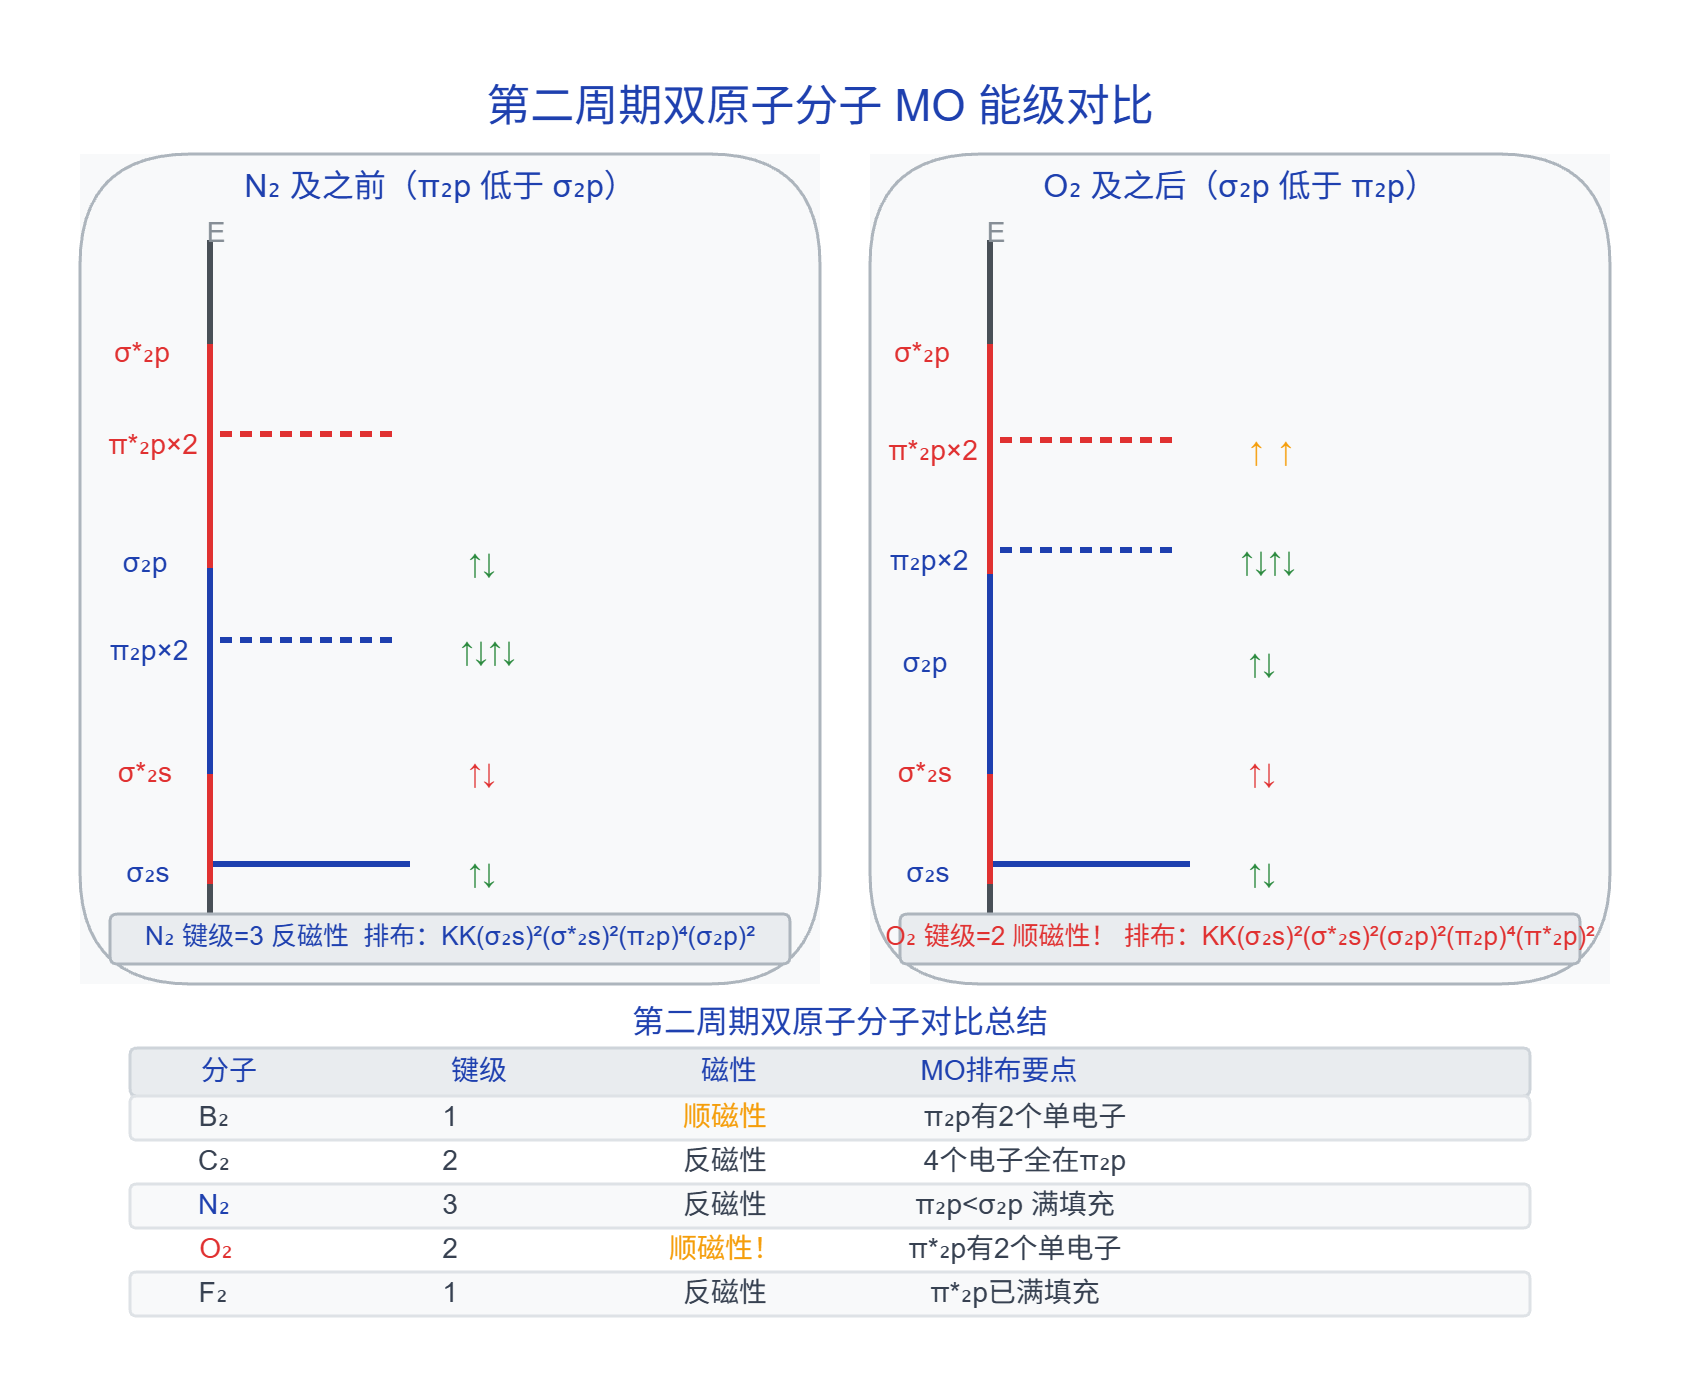
\includegraphics[width=0.9\textwidth,keepaspectratio]{media/h2-energy-curve.jpg}
\caption{图 H2 分子的能量曲线 — 原子轨道组合成成键轨道（σ1s，能量降低）与反键轨道（σ1s}
\end{figure}

\subsubsection{6.2 基本概念}\label{ux57faux672cux6982ux5ff5}

分子轨道理论认为：在分子中，电子不再属于某个特定的原子，而是分布在\textbf{遍及整个分子的分子轨道}中。

{\def\LTcaptype{none} % do not increment counter
\begin{longtable}[]{@{}llll@{}}
\toprule\noalign{}
轨道类型 & 成键方式 & 重叠方式 & 特点 \\
\midrule\noalign{}
\endhead
\bottomrule\noalign{}
\endlastfoot
\textbf{σ 轨道} & 轨道''头对头''重叠 & 沿键轴方向 & 键能大，可旋转 \\
\textbf{π 轨道} & 轨道''肩并肩''重叠 & 垂直于键轴方向 & 键能小，不可旋转 \\
\textbf{δ 轨道} & 轨道''面对面''重叠 & 两个平面 & 仅出现在 d 轨道配合物 \\
\end{longtable}
}

\begin{figure}[H]\centering
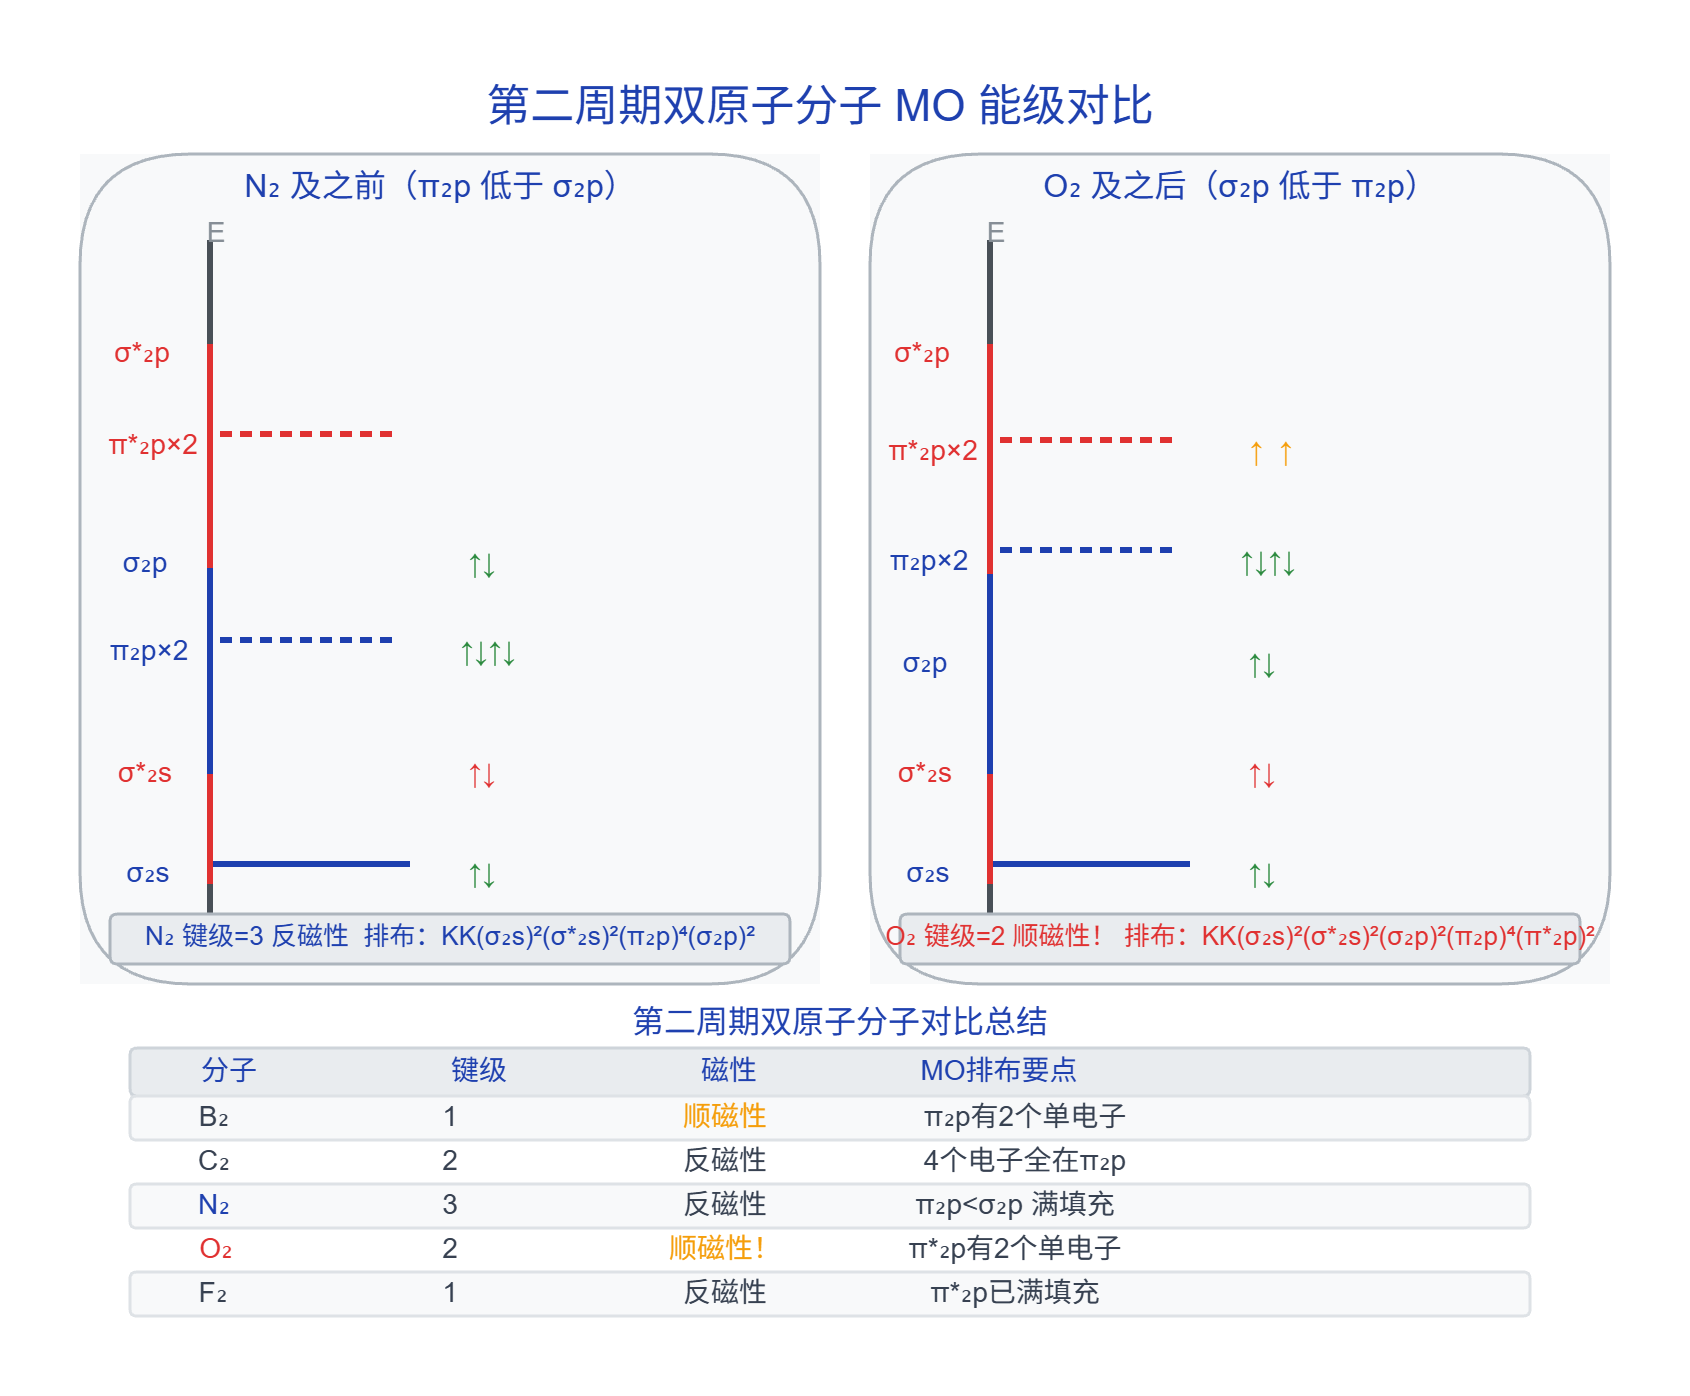
\includegraphics[width=0.9\textwidth,keepaspectratio]{media/sigma-pi-bond-formation.jpg}
\caption{图 σ 键（头对头重叠）与 π 键（肩并肩重叠）的形成方式}
\end{figure}

\subsubsection{6.3 第二周期双原子分子 MO 能级图}\label{ux7b2cux4e8cux5468ux671fux53ccux539fux5b50ux5206ux5b50-mo-ux80fdux7ea7ux56fe}

\textbf{键级公式}：

\[
\text{键级} = \frac{\text{成键电子数} - \text{反键电子数}}{2}
\]

\textbf{两种能级顺序}：

\begin{figure}[H]\centering
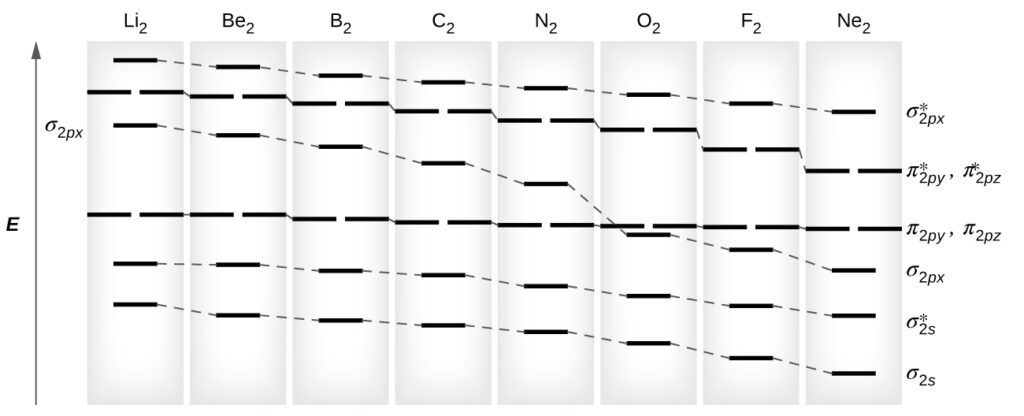
\includegraphics[width=0.9\textwidth,keepaspectratio]{media/mo_diagram_all_second_period.jpg}
\caption{图 第二周期双原子分子 MO 能级图 — 左边为 B2-C2-N2 顺序（s-p 混杂），右边为 O2-F2-Ne2 顺序（无 s-p 混杂）}
\end{figure}

\begin{Shaded}
\begin{Highlighting}[]
\NormalTok{B\textasciitilde{}2\textasciitilde{}、C\textasciitilde{}2\textasciitilde{}、N\textasciitilde{}2\textasciitilde{}（s{-}p 混杂显著）：}
\NormalTok{σ\textasciitilde{}1\textasciitilde{}s \textless{} σ\textasciitilde{}1\textasciitilde{}s* \textless{} σ\textasciitilde{}2\textasciitilde{}s \textless{} σ\textasciitilde{}2\textasciitilde{}s* \textless{} π\textasciitilde{}2\textasciitilde{}pᵧ = π\textasciitilde{}2\textasciitilde{}p\_z \textless{} σ\textasciitilde{}2\textasciitilde{}pₓ \textless{} π\textasciitilde{}2\textasciitilde{}pᵧ* = π\textasciitilde{}2\textasciitilde{}p\_z* \textless{} σ\textasciitilde{}2\textasciitilde{}pₓ*}

\NormalTok{O\textasciitilde{}2\textasciitilde{}、F\textasciitilde{}2\textasciitilde{}、Ne\textasciitilde{}2\textasciitilde{}（s{-}p 混杂可忽略）：}
\NormalTok{σ\textasciitilde{}1\textasciitilde{}s \textless{} σ\textasciitilde{}1\textasciitilde{}s* \textless{} σ\textasciitilde{}2\textasciitilde{}s \textless{} σ\textasciitilde{}2\textasciitilde{}s* \textless{} σ\textasciitilde{}2\textasciitilde{}pₓ \textless{} π\textasciitilde{}2\textasciitilde{}pᵧ = π\textasciitilde{}2\textasciitilde{}p\_z \textless{} π\textasciitilde{}2\textasciitilde{}pᵧ* = π\textasciitilde{}2\textasciitilde{}p\_z* \textless{} σ\textasciitilde{}2\textasciitilde{}pₓ*}
\end{Highlighting}
\end{Shaded}

\textbf{记忆口诀}：``N\textsubscript{2} 及之前 π\textsubscript{2}p 低于 σ\textsubscript{2}p，O\textsubscript{2} 及之后 σ\textsubscript{2}p 低于 π\textsubscript{2}p''

\begin{figure}[H]\centering
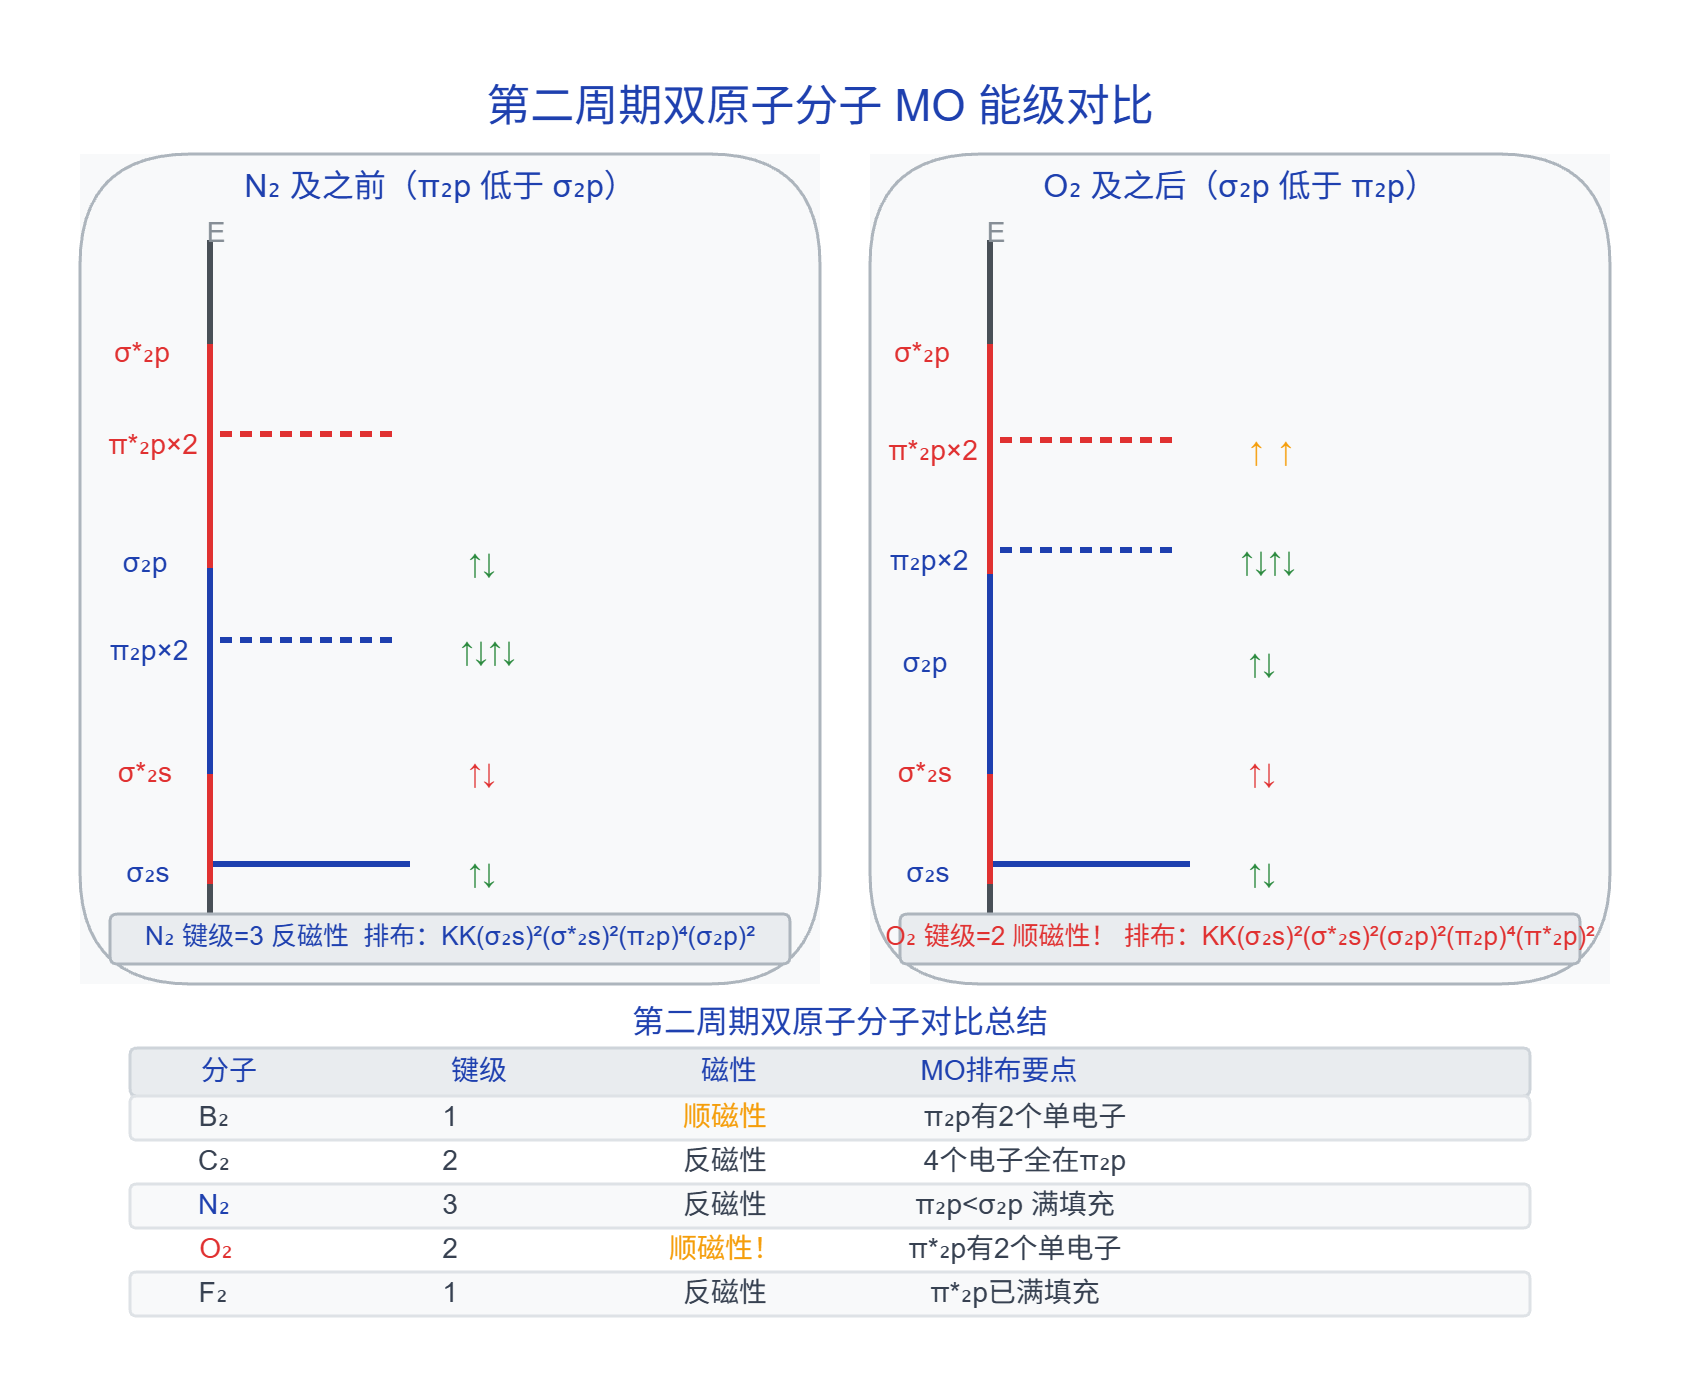
\includegraphics[width=0.9\textwidth,keepaspectratio]{media/第二周期MO能级对比.关系图.png}
\caption{图 第二周期双原子分子 MO 能级对比。左列 N2 型（π2p<σ2p）与右列 O2 型（σ2p<π2p）能级顺序并列对比，底部 B2→F2 键级/磁性总结表。注意 O2 的 π}
\end{figure}

\textbf{为什么有两种顺序？} 当 2s 和 2p 轨道能量差较小时（B\textsubscript{2}、C\textsubscript{2}、N\textsubscript{2}），σ\textsubscript{2}p 与 π\textsubscript{2}p 发生 \textbf{sp 混杂}，σ\textsubscript{2}p 被推高到 π\textsubscript{2}p 之上；当能量差较大时（O\textsubscript{2}、F\textsubscript{2}），无混杂，σ\textsubscript{2}p 在 π\textsubscript{2}p 之下。

\begin{quote}
🧠 \textbf{教学洞察}：sp 混杂是 MO 理论中最容易让人困惑的概念。直观理解：当 2s 和 2p 轨道能量接近时（B、C、N 的 2s/2p 能量差小于 O、F），σ\textsubscript{2}s 和 σ\textsubscript{2}p 会''互相排斥''------σ\textsubscript{2}s 被推低，σ\textsubscript{2}p 被推高，结果 σ\textsubscript{2}p 的能量高于 π\textsubscript{2}p。这就是为什么 N\textsubscript{2} 的能级顺序特殊。\textbf{记忆口诀}：``N\textsubscript{2} 及之前 π\textsubscript{2}p 低于 σ\textsubscript{2}p，O\textsubscript{2} 及之后 σ\textsubscript{2}p 低于 π\textsubscript{2}p''。
\end{quote}

\subsubsection{6.4 典型分子的 MO 电子排布}\label{ux5178ux578bux5206ux5b50ux7684-mo-ux7535ux5b50ux6392ux5e03}

\begin{figure}[H]\centering
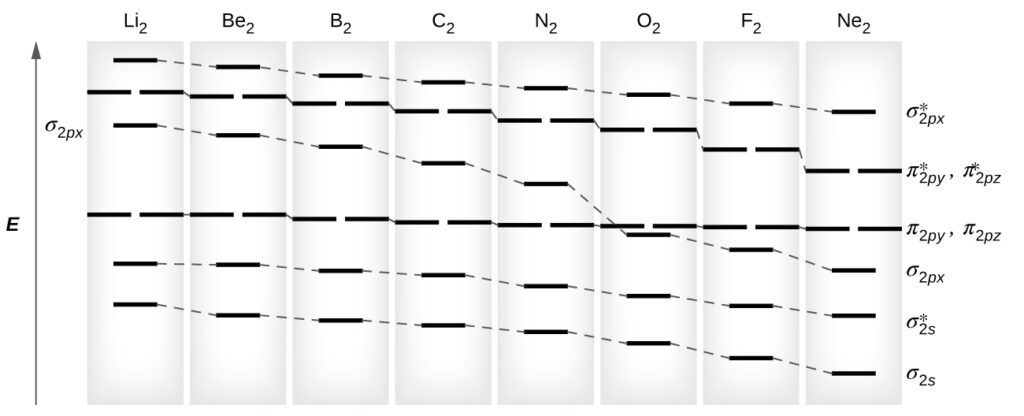
\includegraphics[width=0.9\textwidth,keepaspectratio]{media/mo_diagram_all_second_period.jpg}
\caption{图 O2 的分子轨道能级图 — π2p}
\end{figure}

\begin{figure}[H]\centering
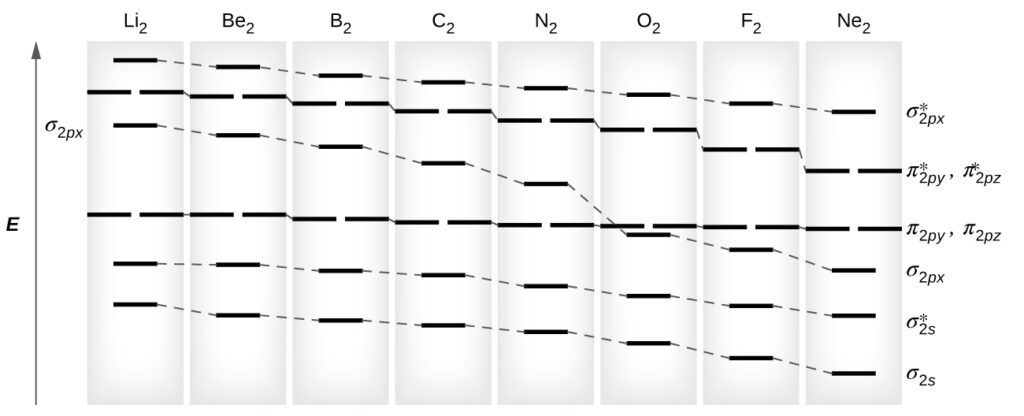
\includegraphics[width=0.9\textwidth,keepaspectratio]{media/mo_diagram_all_second_period.jpg}
\caption{图 第二周期同核双原子分子 MO 电子排布汇总 — 从 B2 到 Ne2 的键级与磁性变化}
\end{figure}

{\def\LTcaptype{none} % do not increment counter
\begin{longtable}[]{@{}
  >{\centering\arraybackslash}p{(\linewidth - 8\tabcolsep) * \real{0.2083}}
  >{\centering\arraybackslash}p{(\linewidth - 8\tabcolsep) * \real{0.2083}}
  >{\raggedright\arraybackslash}p{(\linewidth - 8\tabcolsep) * \real{0.1667}}
  >{\centering\arraybackslash}p{(\linewidth - 8\tabcolsep) * \real{0.2083}}
  >{\centering\arraybackslash}p{(\linewidth - 8\tabcolsep) * \real{0.2083}}@{}}
\toprule\noalign{}
\begin{minipage}[b]{\linewidth}\centering
分子
\end{minipage} & \begin{minipage}[b]{\linewidth}\centering
价电子数
\end{minipage} & \begin{minipage}[b]{\linewidth}\raggedright
电子排布（价层）
\end{minipage} & \begin{minipage}[b]{\linewidth}\centering
键级
\end{minipage} & \begin{minipage}[b]{\linewidth}\centering
磁性
\end{minipage} \\
\midrule\noalign{}
\endhead
\bottomrule\noalign{}
\endlastfoot
B\textsubscript{2} & 6 & \(\sigma_{2s}^2 \sigma_{2s}^{*2} \pi_{2p}^2\) & 1 & 顺磁性（2 个单电子） \\
C\textsubscript{2} & 8 & \(\sigma_{2s}^2 \sigma_{2s}^{*2} \pi_{2p}^4\) & 2 & 反磁性 \\
N\textsubscript{2} & 10 & \(\sigma_{2s}^2 \sigma_{2s}^{*2} \pi_{2p}^4 \sigma_{2p}^2\) & 3 & 反磁性 \\
O\textsubscript{2} & 12 & \(\sigma_{2s}^2 \sigma_{2s}^{*2} \sigma_{2p}^2 \pi_{2p}^4 \pi_{2p}^{*2}\) & 2 & \textbf{顺磁性}（2 个单电子）✅ \\
F\textsubscript{2} & 14 & \(\sigma_{2s}^2 \sigma_{2s}^{*2} \sigma_{2p}^2 \pi_{2p}^4 \pi_{2p}^{*4}\) & 1 & 反磁性 \\
Ne\textsubscript{2} & 16 & 满填 & 0 & 不存在 \\
\end{longtable}
}

相关 KP：分子轨道理论、键级

\begin{quote}
📝 \textbf{练一练}：填写以下第二周期双原子分子的 MO 信息（参考答案在 §十）：
\textbar{} 分子/离子 \textbar{} 价电子数 \textbar{} 电子排布（价层） \textbar{} 键级 \textbar{} 磁性 \textbar{}
\textbar:---:\textbar:---:\textbar:---\textbar:---:\textbar:---:\textbar{}
\textbar{} B\textsubscript{2} \textbar{} 6 \textbar{} \(\sigma_{2s}^2 \sigma_{2s}^{*2} \pi_{2p}^2\) \textbar{} 1 \textbar{} 顺磁性 \textbar{}
\textbar{} C\textsubscript{2} \textbar{} 8 \textbar{} \_\_\_\_ \textbar{} \_\_\_\_ \textbar{} \_\_\_\_ \textbar{}
\textbar{} N\textsubscript{2} \textbar{} 10 \textbar{} \_\_\_\_ \textbar{} \_\_\_\_ \textbar{} \_\_\_\_ \textbar{}
\textbar{} O\textsubscript{2} \textbar{} 12 \textbar{} \_\_\_\_ \textbar{} \_\_\_\_ \textbar{} \_\_\_\_ \textbar{}
\textbar{} O\textsubscript{2}\textsuperscript{-} \textbar{} 13 \textbar{} \_\_\_\_ \textbar{} \_\_\_\_ \textbar{} \_\_\_\_ \textbar{}
\textbar{} O\textsubscript{2}\textsuperscript{2-} \textbar{} 14 \textbar{} \_\_\_\_ \textbar{} \_\_\_\_ \textbar{} \_\_\_\_ \textbar{}
\textbar{} F\textsubscript{2} \textbar{} 14 \textbar{} \_\_\_\_ \textbar{} \_\_\_\_ \textbar{} \_\_\_\_ \textbar{}
\emph{提示：注意 N\textsubscript{2} 和 O\textsubscript{2} 的能级顺序不同！O\textsubscript{2} 体系用 O\textsubscript{2} 的顺序（σ\textsubscript{2}p \textless{} π\textsubscript{2}p），O\textsubscript{2}\textsuperscript{2-} 有 14 个价电子（比 O\textsubscript{2} 多 2 个）→ 填满 π\textsubscript{2}p}。*
\end{quote}

\begin{center}\rule{0.5\linewidth}{0.5pt}\end{center}

\subsection{七、分子间作用力 ------ 从分子到聚集态}\label{ux4e03ux5206ux5b50ux95f4ux4f5cux7528ux529b-ux4eceux5206ux5b50ux5230ux805aux96c6ux6001}

前面六节都在讨论\textbf{单个分子内部}的结构和成键。但化学世界是由大量分子聚集而成的------水为什么是液体（而不是气体）？蜡为什么是固体？为什么 NH\textsubscript{3} 在水中溶解度极大而 PH\textsubscript{3} 极小？

答案就在\textbf{分子之间}的作用力。虽然这些力比化学键弱得多（1--40 kJ/mol 对比 100--800 kJ/mol），但它们决定了物质的\textbf{熔点、沸点、溶解度、表面张力}等一切宏观物理性质。

\begin{quote}
💡 \textbf{为何重要}：分子间力是连接''微观分子结构''与''宏观物理性质''的桥梁。竞赛中约 30\% 的结构化学简答题最终落脚到分子间力解释------比如''为什么 H\textsubscript{2}O 的沸点高于 H\textsubscript{2}S''\,``为什么 NH\textsubscript{3} 在水中溶解度极大''。
\end{quote}

\subsubsection{7.1 分子间力概述}\label{ux5206ux5b50ux95f4ux529bux6982ux8ff0}

分子间作用力虽然弱于化学键（\textasciitilde1--40 kJ/mol vs 100--800 kJ/mol），但决定物质的\textbf{熔点、沸点、溶解度}等物理性质。

{\def\LTcaptype{none} % do not increment counter
\begin{longtable}[]{@{}llcll@{}}
\toprule\noalign{}
类型 & 本质 & 强度 & 存在范围 & 实例 \\
\midrule\noalign{}
\endhead
\bottomrule\noalign{}
\endlastfoot
\textbf{色散力} & 瞬时偶极 & 最弱 & 所有分子/原子 & 稀有气体液化 \\
\textbf{诱导力} & 永久偶极诱导 & 较弱 & 极性+非极性 & O\textsubscript{2} 溶于水 \\
\textbf{取向力} & 永久偶极间 & 较强 & 极性分子间 & HCl、H\textsubscript{2}O \\
\end{longtable}
}

记忆口诀：\textbf{``极性有取向，极化生诱导，万物有色散''}

\begin{figure}[H]\centering
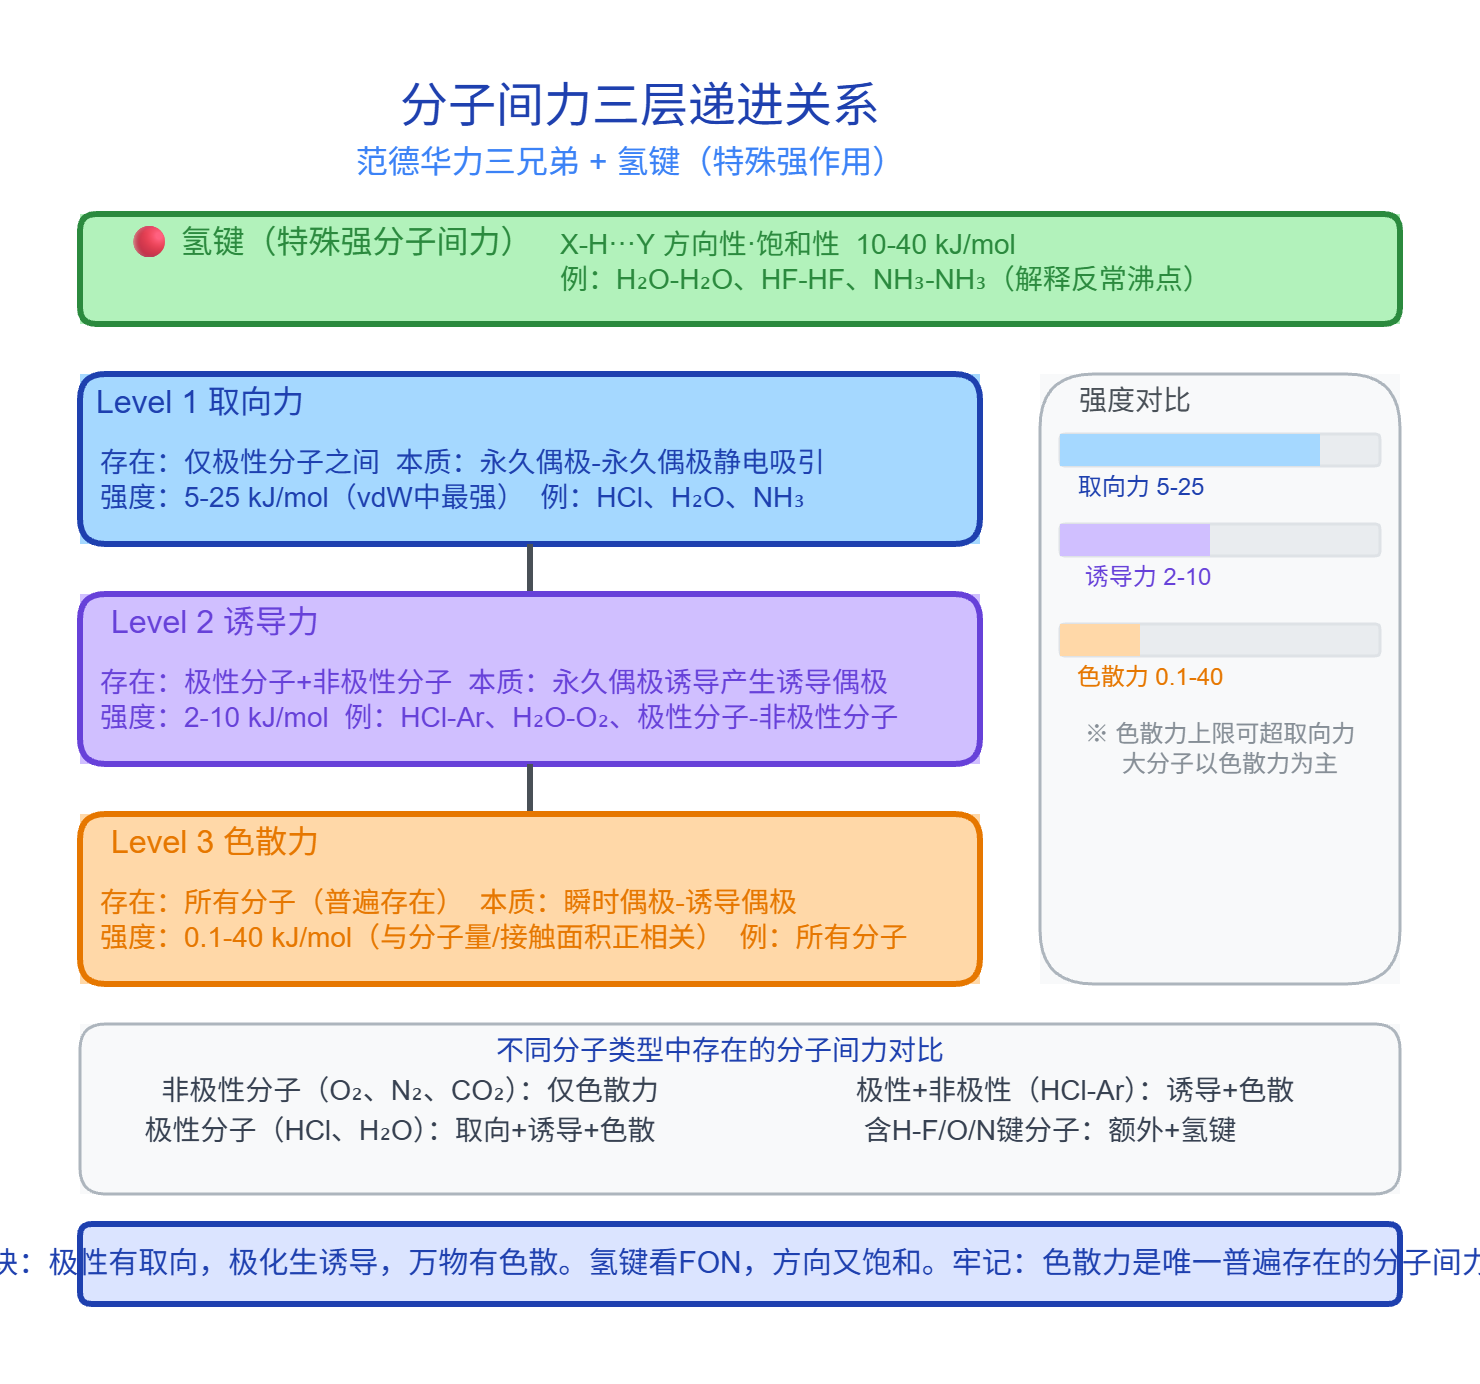
\includegraphics[width=0.9\textwidth,keepaspectratio]{media/分子间力三层递进.关系图.png}
\caption{图 分子间力三层递进关系。上方为氢键（特殊强作用），下方为范德华力三兄弟（取向力→诱导力→色散力），右侧为强度对比条，底部为不同分子类型中的分子间力存在情况和记忆口诀。}
\end{figure}

\subsubsection{7.2 氢键}\label{ux6c22ux952e}

\textbf{形成条件}（缺一不可）：
1. 有 X-H 键（X = F、O、N）
2. Y 上有孤对电子（Y = F、O、N）
3. X、Y 电负性大、半径小

\begin{quote}
🧠 \textbf{教学洞察}：氢键的本质是一种\textbf{特殊的偶极-偶极相互作用}，强度介于化学键和范德华力之间。学生最常问的问题是------``为什么 NH\textsubscript{3} 的沸点比 H\textsubscript{2}O 低？NH\textsubscript{3} 也能形成氢键啊！''答案是：\textbf{每个 H\textsubscript{2}O 可以形成 4 个氢键（2 个 O-H 供体 + 2 对孤对受体），而 NH\textsubscript{3} 只能形成 2 个（3 个 N-H 供体但只有 1 对孤对受体）}。水中的氢键网络更加立体和完整，因此破坏它需要更多能量。
\end{quote}

\begin{quote}
⚠️ \textbf{易错点}：氢键的\textbf{方向性}（X-H···Y 趋向于 180°）和\textbf{饱和性}（每个 X-H 只能与一个 Y 形成氢键）经常被忽视。判断一个分子能否形成氢键时，记住：\textbf{必须同时有 X-H（供体）和 Y 上的孤对电子（受体）}------CH\textsubscript{4} 虽然有 C-H 键，但 C 的电负性太小（2.5），不能形成氢键。
\end{quote}

\textbf{氢键强度序列}：

\[
\text{F-H} \cdots \text{F} > \text{O-H} \cdots \text{O} > \text{O-H} \cdots \text{N} > \text{N-H} \cdots \text{O} > \text{N-H} \cdots \text{N}
\]

\textbf{氢键的特点}：
- \textbf{方向性}：X-H···Y 趋向于直线排列（\textasciitilde180°）
- \textbf{饱和性}：每个 X-H 只能与一个 Y 形成氢键

\textbf{氢键对物性的影响}：

{\def\LTcaptype{none} % do not increment counter
\begin{longtable}[]{@{}lll@{}}
\toprule\noalign{}
性质 & 效应 & 经典例证 \\
\midrule\noalign{}
\endhead
\bottomrule\noalign{}
\endlastfoot
沸点 & 含氢键的分子沸点大幅升高 & H\textsubscript{2}O(100°C) vs H\textsubscript{2}S(-60°C) \\
溶解度 & 溶质与溶剂形成氢键→溶解度增大 & NH\textsubscript{3} 在水中溶解度极大 \\
密度 & 冰中氢键形成空旷结构→密度小于水 & 冰浮于水上 \\
\end{longtable}
}

相关 KP：分子间力、氢键、范德华力

\begin{center}\rule{0.5\linewidth}{0.5pt}\end{center}

\subsection{八、典型例题}\label{ux516bux5178ux578bux4f8bux9898}

\subsubsection{例1 Lewis 结构 + 形式电荷 ⭐⭐}\label{ux4f8b1-lewis-ux7ed3ux6784-ux5f62ux5f0fux7535ux8377}

\textbf{题目}：画出 XeF\textsubscript{2} 的 Lewis 结构，标出形式电荷，判断中心原子的杂化方式与分子构型。

\textbf{思路分析}：
1. 先算总价电子数：Xe(8) + F(1×2) = 10
2. Xe 为中心原子，2 个 F 在端基
3. 判断是否满足八隅体规则------Xe 为第三周期元素，可超八隅体

\textbf{完整解答}：

总价电子数 = 10。

骨架 F-Xe-F，2 个单键用去 4e\textsuperscript{-}，剩余 6e\textsuperscript{-}。

Xe 周围：2 个单键（4e\textsuperscript{-}）+ 3 对孤对（6e\textsuperscript{-}）= 10e\textsuperscript{-}

形式电荷：Xe(8 - 6 - 2/2 = -1)，F(7 - 6 - 2/2 = 0)

修正：实际 XeF\textsubscript{2} 的 Xe 形式电荷为 0，F 为 0。最优 Lewis 结构中 Xe 周围有 3 对孤对。

VSEPR 分析：Xe 有 2 个 σ 键 + 3 对孤对 = 5 个电子对 → 三角双锥排布 → AX\textsubscript{2}E\textsubscript{3} → \textbf{直线形}

杂化：sp\textsuperscript{3}d

\textbf{答案}：XeF\textsubscript{2} 为直线形分子，中心 Xe 采用 sp\textsuperscript{3}d 杂化，Lewis 结构中 Xe 周围有 3 对孤对。

\begin{center}\rule{0.5\linewidth}{0.5pt}\end{center}

\subsubsection{例2 VSEPR + 杂化 + 反常构型 ⭐⭐⭐}\label{ux4f8b2-vsepr-ux6742ux5316-ux53cdux5e38ux6784ux578b}

\textbf{题目}：比较 (CH\textsubscript{3})\textsubscript{3}N 和 (SiH\textsubscript{3})\textsubscript{3}N 的分子构型，解释差异的原因。

\textbf{思路分析}：
1. 分别判断 N 的杂化方式
2. (CH\textsubscript{3})\textsubscript{3}N 中 N 的孤对电子在 sp\textsuperscript{3} 杂化轨道中，分子为三角锥形
3. (SiH\textsubscript{3})\textsubscript{3}N 中 Si 有 3d 空轨道，可接受 N 的孤对电子

\textbf{完整解答}：

{\def\LTcaptype{none} % do not increment counter
\begin{longtable}[]{@{}
  >{\raggedright\arraybackslash}p{(\linewidth - 8\tabcolsep) * \real{0.1905}}
  >{\raggedright\arraybackslash}p{(\linewidth - 8\tabcolsep) * \real{0.1905}}
  >{\raggedright\arraybackslash}p{(\linewidth - 8\tabcolsep) * \real{0.1905}}
  >{\centering\arraybackslash}p{(\linewidth - 8\tabcolsep) * \real{0.2381}}
  >{\raggedright\arraybackslash}p{(\linewidth - 8\tabcolsep) * \real{0.1905}}@{}}
\toprule\noalign{}
\begin{minipage}[b]{\linewidth}\raggedright
分子
\end{minipage} & \begin{minipage}[b]{\linewidth}\raggedright
预测构型
\end{minipage} & \begin{minipage}[b]{\linewidth}\raggedright
实际构型
\end{minipage} & \begin{minipage}[b]{\linewidth}\centering
N 的杂化
\end{minipage} & \begin{minipage}[b]{\linewidth}\raggedright
解释
\end{minipage} \\
\midrule\noalign{}
\endhead
\bottomrule\noalign{}
\endlastfoot
(CH\textsubscript{3})\textsubscript{3}N & 三角锥形 & 三角锥形 & sp\textsuperscript{3} & N 的孤对电子在杂化轨道中，C 没有 3d 空轨道 \\
(SiH\textsubscript{3})\textsubscript{3}N & 三角锥形（无离域） & \textbf{平面三角形} & sp\textsuperscript{2} & N 的孤对电子离域到 Si 的 3d 空轨道 → d-pπ 键 → N 从 sp\textsuperscript{3} 变为 sp\textsuperscript{2} \\
\end{longtable}
}

\textbf{答案}：
- (CH\textsubscript{3})\textsubscript{3}N：三角锥形，N 为 sp\textsuperscript{3} 杂化
- (SiH\textsubscript{3})\textsubscript{3}N：平面三角形，N 为 sp\textsuperscript{2} 杂化（孤对电子参与 d-pπ 离域）

\begin{center}\rule{0.5\linewidth}{0.5pt}\end{center}

\subsubsection{例3 MO + 键级 + 磁性判断 ⭐⭐⭐}\label{ux4f8b3-mo-ux952eux7ea7-ux78c1ux6027ux5224ux65ad}

\textbf{题目}：用分子轨道理论比较 N\textsubscript{2}、O\textsubscript{2}、O\textsubscript{2}\textsuperscript{-} 的键级与磁性。

\textbf{思路分析}：
1. 画出 N\textsubscript{2} 和 O\textsubscript{2} 的 MO 能级图
2. 注意 N\textsubscript{2} 和 O\textsubscript{2} 的能级顺序不同（sp 混杂效应）
3. O\textsubscript{2}\textsuperscript{-} 比 O\textsubscript{2} 多 1 个电子 → 填入反键轨道

\textbf{完整解答}：

\textbf{N\textsubscript{2}（10 个价电子，N 之前能级顺序）}：
\[
\sigma_{2s}^2 \sigma_{2s}^{*2} \pi_{2p}^4 \sigma_{2p}^2
\]
- 键级 = (8 - 2)/2 = \textbf{3}（N≡N 三键）
- 无单电子 → \textbf{反磁性}

\textbf{O\textsubscript{2}（12 个价电子，O 之后能级顺序）}：
\[
\sigma_{2s}^2 \sigma_{2s}^{*2} \sigma_{2p}^2 \pi_{2p}^4 \pi_{2p}^{*2}
\]
- 键级 = (8 - 4)/2 = \textbf{2}（O=O 双键）
- 有 2 个单电子 → \textbf{顺磁性} ✅（实验证实！）

\textbf{O\textsubscript{2}\textsuperscript{-}（13 个价电子）}：
\[
\sigma_{2s}^2 \sigma_{2s}^{*2} \sigma_{2p}^2 \pi_{2p}^4 \pi_{2p}^{*3}
\]
- 键级 = (8 - 5)/2 = \textbf{1.5}
- 有 1 个单电子 → \textbf{顺磁性}

\textbf{稳定性}：N\textsubscript{2} \textgreater{} O\textsubscript{2} \textgreater{} O\textsubscript{2}\textsuperscript{-}（键级越大越稳定）

\begin{center}\rule{0.5\linewidth}{0.5pt}\end{center}

\subsubsection{例4 分子间力 + 氢键 ⭐⭐}\label{ux4f8b4-ux5206ux5b50ux95f4ux529b-ux6c22ux952e}

\textbf{题目}：解释以下实验现象：
(1) H\textsubscript{2}O 的沸点（100°C）远高于 H\textsubscript{2}S（-60°C）
(2) NH\textsubscript{3} 在水中的溶解度极大，而 PH\textsubscript{3} 溶解度很小

\textbf{思路分析}：
1. 沸点差异 → 分子间作用力类型
2. 溶解度差异 → 溶质-溶剂间能否形成氢键

\textbf{完整解答}：

\begin{enumerate}
\def\labelenumi{(\arabic{enumi})}
\tightlist
\item
  \textbf{H\textsubscript{2}O vs H\textsubscript{2}S 沸点}：
\end{enumerate}

\begin{itemize}
\tightlist
\item
  H\textsubscript{2}O 分子间能形成\textbf{氢键}（O-H···O），需要额外能量克服
\item
  H\textsubscript{2}S 分子间仅存在范德华力（色散力为主），比氢键弱得多
\item
  虽然 H\textsubscript{2}S 分子量更大（色散力更大），但氢键的贡献主导 → H\textsubscript{2}O 沸点反常高
\end{itemize}

\begin{enumerate}
\def\labelenumi{(\arabic{enumi})}
\setcounter{enumi}{1}
\tightlist
\item
  \textbf{NH\textsubscript{3} vs PH\textsubscript{3} 溶解度}：
\end{enumerate}

\begin{itemize}
\tightlist
\item
  NH\textsubscript{3} 分子中的 N-H 键可与 H\textsubscript{2}O 的 O-H 形成\textbf{氢键}（N-H···O 和 O-H···N），溶解度极大
\item
  PH\textsubscript{3} 分子中 P 的电负性小（2.1），不能形成氢键，仅靠范德华力溶解 → 溶解度很小
\end{itemize}

\begin{center}\rule{0.5\linewidth}{0.5pt}\end{center}

\subsubsection{\texorpdfstring{例5 SO\textsubscript{2} 的结构综合推断 ⭐⭐⭐⭐}{例5 SO2 的结构综合推断 ⭐⭐⭐⭐}}\label{ux4f8b5-so2-ux7684ux7ed3ux6784ux7efcux5408ux63a8ux65ad}

\textbf{题目}：SO\textsubscript{2} 是一种常见的 V 形分子，已知其 S-O 键长（143 pm）介于 S-O 单键（\textasciitilde157 pm）和 S=O 双键（\textasciitilde122 pm）之间。

\begin{enumerate}
\def\labelenumi{(\arabic{enumi})}
\tightlist
\item
  画出 SO\textsubscript{2} 的 Lewis 结构（考虑形式电荷），写出可能的共振结构。
\item
  用 VSEPR 理论预测 SO\textsubscript{2} 的分子构型和键角。
\item
  判断 S 的杂化方式。
\item
  SO\textsubscript{2} 中是否存在离域π键？若存在，写出 πₙᵐ 表示并分析电子来源。
\item
  根据以上分析解释为什么 S-O 键长介于单键和双键之间。
\end{enumerate}

\textbf{思路分析}：
1. 先算总价电子数：S(6) + O(6×2) = 18。骨架 O-S-O。
2. 2 个 S-O 单键用去 4e\textsuperscript{-}，剩余 14e\textsuperscript{-} → 先满足 2 个 O（各 6e\textsuperscript{-}）→ 用去 12e\textsuperscript{-}，剩余 2e\textsuperscript{-} → S 上 1 对孤对
3. S 只有 6e\textsuperscript{-}（2 个单键 + 1 对孤对）→ 不满足八隅体 → 改为双键

\textbf{完整解答}：

\begin{enumerate}
\def\labelenumi{(\arabic{enumi})}
\tightlist
\item
  \textbf{Lewis 结构}：
\end{enumerate}

SO\textsubscript{2} 有两种主要共振结构：
- \textbf{结构 A}：S=O（双键）+ S-O\textsuperscript{-}（单键），S 形式电荷 +1，双键 O 形式电荷 0，单键 O\textsuperscript{-} 形式电荷 -1
- \textbf{结构 B}：S-O\textsuperscript{-}（单键）+ S=O（双键），S 形式电荷 +1，与结构 A 对称等价

总价电子数：18，S 满足八隅体（共 3 个电子对区域：2 个 σ 键 + 1 对孤对）。

\begin{enumerate}
\def\labelenumi{(\arabic{enumi})}
\setcounter{enumi}{1}
\tightlist
\item
  \textbf{VSEPR 分析}：
\end{enumerate}

\begin{itemize}
\tightlist
\item
  S 周围：2 个 σ 键 + 1 对孤对 = 3 个电子对区域
\item
  AX\textsubscript{2}E → 理想排布为平面三角形 → 孤对占据一个顶点 → 实际构型为 \textbf{V 形}
\item
  键角 \textless{} 120°（孤对-成键排斥 \textgreater{} 成键-成键排斥），实验值 \textasciitilde119°
\end{itemize}

\begin{enumerate}
\def\labelenumi{(\arabic{enumi})}
\setcounter{enumi}{2}
\tightlist
\item
  \textbf{杂化判断}：
\end{enumerate}

\begin{itemize}
\tightlist
\item
  S 有 3 个电子对区域（2 σ 键 + 1 孤对）→ \textbf{sp\textsuperscript{2} 杂化}
\item
  剩余 1 个未杂化的 3p 轨道垂直于分子平面
\end{itemize}

\begin{enumerate}
\def\labelenumi{(\arabic{enumi})}
\setcounter{enumi}{3}
\tightlist
\item
  \textbf{离域π键}：
\end{enumerate}

\begin{itemize}
\tightlist
\item
  S 为 sp\textsuperscript{2} 杂化 → 剩余垂直 p 轨道
\item
  2 个 O 也各有 1 个垂直 p 轨道（与 S 的 p 轨道平行）
\item
  电子计数：S 提供 1 个 p 电子（因 SO\textsubscript{2} 中 S 有 1 个未成对电子）？实际上 SO\textsubscript{2} 的离域π键计法：

  \begin{itemize}
  \tightlist
  \item
    S 在 sp\textsuperscript{2} 杂化后 3p 轨道上有 2 个电子（S 价电子 6 - 2 个 σ 键 - 1 对孤对 = 剩余 2e\textsuperscript{-}）
  \item
    但离域π键中 S 的 p 轨道实际提供 2 个电子（孤对）
  \item
    2 个 O 各提供 1 个 p 电子（共 2e\textsuperscript{-}）
  \item
    共 4e\textsuperscript{-} 在 3 个原子上离域
  \end{itemize}
\item
  \textbf{π\textsubscript{3}\textsuperscript{4}} 离域π键（三个原子参与，四个电子离域）
\end{itemize}

\begin{enumerate}
\def\labelenumi{(\arabic{enumi})}
\setcounter{enumi}{4}
\tightlist
\item
  \textbf{键长解释}：
\end{enumerate}

\begin{itemize}
\tightlist
\item
  两个共振结构等价 → S-O 键级为 (1 + 2)/2 = 1.5
\item
  键级 1.5 介于单键(1)和双键(2)之间 → 键长 143 pm 介于 S-O (157 pm) 和 S=O (122 pm) 之间
\item
  电子离域使体系能量降低，结构更稳定
\end{itemize}

\textbf{答案}：(1) 两种共振结构；(2) V 形，键角\textasciitilde119°；(3) sp\textsuperscript{2} 杂化；(4) 存在 π\textsubscript{3}\textsuperscript{4}；(5) S-O 键级为 1.5。

\begin{center}\rule{0.5\linewidth}{0.5pt}\end{center}

\subsubsection{例6 异核双原子分子 CO 的 MO 分析 ⭐⭐⭐⭐}\label{ux4f8b6-ux5f02ux6838ux53ccux539fux5b50ux5206ux5b50-co-ux7684-mo-ux5206ux6790}

\textbf{题目}：CO 是初赛高频考点。它与 N\textsubscript{2} 等电子（均为 14 价电子，2 个原子），但 CO 与过渡金属的配位能力远强于 N\textsubscript{2}。

\begin{enumerate}
\def\labelenumi{(\arabic{enumi})}
\tightlist
\item
  画出 CO 的 MO 能级图（参照 N\textsubscript{2} 的能级顺序，因 s-p 混杂显著）。
\item
  计算 CO 的键级并判断磁性。
\item
  写出 CO 的 Lewis 结构。它含有几个配位键？
\item
  用 MO 理论解释：为什么 CO 的配位能力强于 N\textsubscript{2}？
\end{enumerate}

\textbf{思路分析}：
1. CO 与 N\textsubscript{2} 等电子、同原子数 → MO 能级图相似
2. 但 C 和 O 能量不同 → 分子轨道在两端原子上的电子密度分布不对称

\textbf{完整解答}：

\begin{enumerate}
\def\labelenumi{(\arabic{enumi})}
\tightlist
\item
  \textbf{CO 的 MO 能级图}（类似 N\textsubscript{2}，s-p 混杂显著）：
\end{enumerate}

\begin{verbatim}
σ~1~s < σ~1~s* < σ~2~s < σ~2~s* < π~2~pᵧ = π~2~p_z < σ~2~pₓ < π~2~pᵧ* = π~2~p_z* < σ~2~pₓ*
\end{verbatim}

CO 的 14 个价电子排布：
\[
\sigma_{1s}^2 \sigma_{1s}^{*2} \sigma_{2s}^2 \sigma_{2s}^{*2} \pi_{2p}^4 \sigma_{2p}^2
\]

\begin{enumerate}
\def\labelenumi{(\arabic{enumi})}
\setcounter{enumi}{1}
\tightlist
\item
  \textbf{键级与磁性}：
\end{enumerate}

\begin{itemize}
\tightlist
\item
  键级 = (成键电子 - 反键电子) / 2 = (10 - 4) / 2 = \textbf{3}（C≡O 三键）
\item
  所有电子均成对 → \textbf{反磁性}
\end{itemize}

\begin{enumerate}
\def\labelenumi{(\arabic{enumi})}
\setcounter{enumi}{2}
\tightlist
\item
  \textbf{Lewis 结构}：
\end{enumerate}

\begin{itemize}
\tightlist
\item
  CO 的 Lewis 结构可以写为：\(\mathrm{:C≡O:}\)
\item
  计算形式电荷：C(4 - 2 - 6/2 = -1)，O(6 - 2 - 6/2 = +1)
\item
  其中含 \textbf{1 个配位键}（O 提供孤对电子给 C）
\item
  更好的解释：三个共价键中，一个是 O→C 配位键
\end{itemize}

\begin{enumerate}
\def\labelenumi{(\arabic{enumi})}
\setcounter{enumi}{3}
\tightlist
\item
  \textbf{CO 配位能力更强的 MO 解释}：
\end{enumerate}

CO 与过渡金属配位时，两个因素起关键作用：

\textbf{σ 给予}：
- CO 的 σ\textsubscript{2}p（HOMO）在 C 端的电子密度分布系数更大（因 C 的电负性小于 O，2p 轨道能量更高）
- 意味着 σ\textsubscript{2}p 轨道在 C 端有''突出''的电子云 → C 端的孤对电子更容易向金属的空 d 轨道配位
- 对比 N\textsubscript{2}：N\textsubscript{2} 的 σ\textsubscript{2}p 轨道两端对称，给予能力不如 CO

\textbf{π 反馈}：
- CO 的反键轨道 π\textsubscript{2}p\emph{（LUMO）在 C 端也有更大的系数
- 金属的 d 电子可以反馈到 CO 的 π\textsubscript{2}p} 空轨道 → 形成 d→π* 反馈π键
- σ-给予 + π-反馈协同增强 → 形成稳定的配位键

\textbf{综合}：C≡O 的配位能力强于 N≡N，正是因为其 σ 给予能力更强（C 端电子密度不对称），且 π* 反馈轨道更容易接近。

\textbf{竞赛考点}：CO 是初赛结构化学和配位化学的核心衔接点。注意 CO 与金属配位时常用 C 端而非 O 端------因 C 端 σ 给予能力更强。

\begin{center}\rule{0.5\linewidth}{0.5pt}\end{center}

\subsubsection{例7 综合：未知物种的结构推断 ⭐⭐⭐⭐⭐}\label{ux4f8b7-ux7efcux5408ux672aux77e5ux7269ux79cdux7684ux7ed3ux6784ux63a8ux65ad}

\textbf{题目}：一未知离子 X 的化学式为 NCO\textsuperscript{-}（氰酸根离子），已知它有三种可能的共振结构。

\begin{enumerate}
\def\labelenumi{(\arabic{enumi})}
\tightlist
\item
  画出 NCO\textsuperscript{-} 中所有可能满足八隅体规则的共振结构（N 为端基原子，C 为中心原子），标出形式电荷，选出最优结构。
\item
  用 VSEPR 理论预测 NCO\textsuperscript{-} 的分子构型，判断中心 C 的杂化方式。
\item
  判断 NCO\textsuperscript{-} 与哪些分子/离子等电子，写出 2-3 个等电子体。
\item
  若将 NCO\textsuperscript{-} 中的 N 换为 S（得到 SCO），SCO 的构型是否与 NCO\textsuperscript{-} 相同？键角会如何变化？
\end{enumerate}

\textbf{思路分析}：
1. 计算总价电子数：N(5) + C(4) + O(6) + 1(负电荷) = 16
2. 线性骨架 N-C-O，3 个原子，16 个价电子
3. 等电子体法：16e\textsuperscript{-} + 3 原子 → 参照 CO\textsubscript{2}（16e\textsuperscript{-}，3 原子）

\textbf{完整解答}：

\begin{enumerate}
\def\labelenumi{(\arabic{enumi})}
\tightlist
\item
  \textbf{共振结构}：
\end{enumerate}

{\def\LTcaptype{none} % do not increment counter
\begin{longtable}[]{@{}
  >{\raggedright\arraybackslash}p{(\linewidth - 10\tabcolsep) * \real{0.1538}}
  >{\raggedright\arraybackslash}p{(\linewidth - 10\tabcolsep) * \real{0.1538}}
  >{\centering\arraybackslash}p{(\linewidth - 10\tabcolsep) * \real{0.1923}}
  >{\centering\arraybackslash}p{(\linewidth - 10\tabcolsep) * \real{0.1923}}
  >{\raggedright\arraybackslash}p{(\linewidth - 10\tabcolsep) * \real{0.1538}}
  >{\raggedright\arraybackslash}p{(\linewidth - 10\tabcolsep) * \real{0.1538}}@{}}
\toprule\noalign{}
\begin{minipage}[b]{\linewidth}\raggedright
结构
\end{minipage} & \begin{minipage}[b]{\linewidth}\raggedright
Lewis 表示
\end{minipage} & \begin{minipage}[b]{\linewidth}\centering
N-C
\end{minipage} & \begin{minipage}[b]{\linewidth}\centering
C-O
\end{minipage} & \begin{minipage}[b]{\linewidth}\raggedright
形式电荷
\end{minipage} & \begin{minipage}[b]{\linewidth}\raggedright
说明
\end{minipage} \\
\midrule\noalign{}
\endhead
\bottomrule\noalign{}
\endlastfoot
A & N≡C-O\textsuperscript{-} & 三键 & 单键 & N≡C(0), C-O\textsuperscript{-}(-1 on O) & 三者中次优 \\
B & \textsuperscript{-}N=C=O & 双键 & 双键 & \textsuperscript{-}N(-1 on N), C=O(0) & 三者中最优 \\
C & N\textsuperscript{-}-C≡O\textsuperscript{+} & 单键 & 三键 & N\textsuperscript{-}(-1 on N), C≡O\textsuperscript{+}(+1 on O) & 三者中最差（相邻正负电荷） \\
\end{longtable}
}

\textbf{最优结构}：\textbf{结构 B}（\textsuperscript{-}N=C=O）
- 形式电荷之和最小（-1 + 0 + 0 = -1）
- 负电荷在电负性较大的 N 原子上
- 无相邻同号电荷

\begin{enumerate}
\def\labelenumi{(\arabic{enumi})}
\setcounter{enumi}{1}
\tightlist
\item
  \textbf{VSEPR 与杂化}：
\end{enumerate}

\begin{itemize}
\tightlist
\item
  C 为 sp 杂化（2 个 σ 键 + 0 对孤对 → 2 个电子对区域 → sp 杂化 → 直线形）
\item
  分子构型：\textbf{直线形}（键角 180°）
\end{itemize}

\begin{enumerate}
\def\labelenumi{(\arabic{enumi})}
\setcounter{enumi}{2}
\tightlist
\item
  \textbf{等电子体}（16 e\textsuperscript{-}，3 原子）：
\end{enumerate}

\begin{itemize}
\tightlist
\item
  \textbf{CO\textsubscript{2}}（O=C=O）
\item
  \textbf{N\textsubscript{2}O}（N≡N\textsuperscript{+}-O\textsuperscript{-} 或 \textsuperscript{-}N=N\textsuperscript{+}=O）
\item
  \textbf{NO\textsubscript{2}\textsuperscript{+}}（{[}O=N=O{]}\textsuperscript{+}，硝酰阳离子）
\item
  \textbf{N\textsubscript{3}\textsuperscript{-}}（叠氮离子，{[}N=N=N{]}\textsuperscript{-}）
\end{itemize}

\begin{enumerate}
\def\labelenumi{(\arabic{enumi})}
\setcounter{enumi}{3}
\tightlist
\item
  \textbf{NCO\textsuperscript{-} vs SCO}：
\end{enumerate}

\begin{itemize}
\tightlist
\item
  SCO（羰基硫）：S 替换 N 后，总价电子数不变（16），3 原子
\item
  构型：仍为 \textbf{直线形}（与 NCO\textsuperscript{-} 相同）
\item
  键角变化：仍为 180°（直线形无变化）
\item
  \textbf{键长变化}：S 的原子半径大于 N → S-C 键长大于 N-C 键长
\item
  S 的电负性（2.6）小于 N（3.0）→ S-C 键极性小于 N-C 键
\end{itemize}

\textbf{答案}：(1) 最优结构为 \textsuperscript{-}N=C=O；(2) 直线形，sp 杂化；(3) CO\textsubscript{2}、N\textsubscript{2}O、NO\textsubscript{2}\textsuperscript{+} 等；(4) 构型相同（直线形），S-C 键更长。

\textbf{竞赛要点}：等电子体原理是竞赛推断题中最强大的工具之一。对于未知物种，先算价电子数 + 原子数 → 找等电子体 → 套用已知结构。本题的 NCO\textsuperscript{-} 与 CO\textsubscript{2} 等电子（16e\textsuperscript{-}/3 原子），因此构型也为直线形。

\begin{center}\rule{0.5\linewidth}{0.5pt}\end{center}

\subsection{九、方法总结 · 结构预测工具链}\label{ux4e5dux65b9ux6cd5ux603bux7ed3-ux7ed3ux6784ux9884ux6d4bux5de5ux5177ux94fe}

\subsubsection{9.1 分子结构预测流程图}\label{ux5206ux5b50ux7ed3ux6784ux9884ux6d4bux6d41ux7a0bux56fe}

\begin{figure}[H]\centering
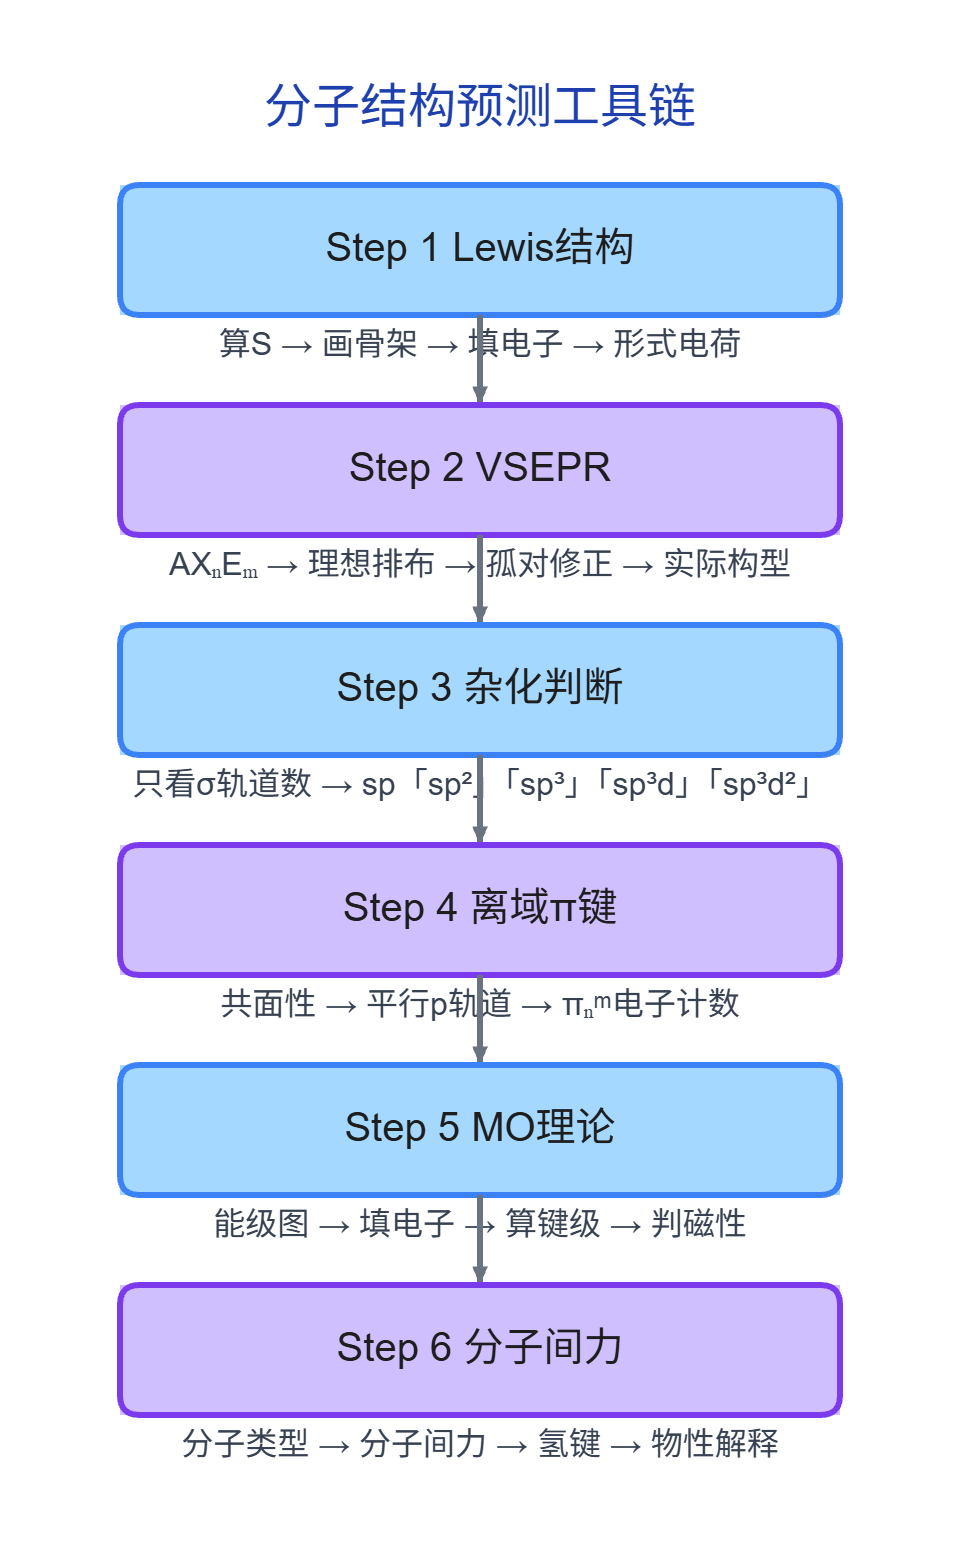
\includegraphics[width=0.9\textwidth,keepaspectratio]{media/分子结构预测工具链.流程图.png}

\end{figure}

\emph{图 分子结构预测工具链 --- 从化学式到分子间作用力的完整预测流程。点击图中各步骤可跳转到对应章节。该流程贯穿整个分子结构内容的学习，建议每次解题时按此顺序逐步推进。}

\subsubsection{9.2 核心速查表}\label{ux6838ux5fc3ux901fux67e5ux8868}

{\def\LTcaptype{none} % do not increment counter
\begin{longtable}[]{@{}
  >{\raggedright\arraybackslash}p{(\linewidth - 6\tabcolsep) * \real{0.2500}}
  >{\raggedright\arraybackslash}p{(\linewidth - 6\tabcolsep) * \real{0.2500}}
  >{\raggedright\arraybackslash}p{(\linewidth - 6\tabcolsep) * \real{0.2500}}
  >{\raggedright\arraybackslash}p{(\linewidth - 6\tabcolsep) * \real{0.2500}}@{}}
\toprule\noalign{}
\begin{minipage}[b]{\linewidth}\raggedright
工具
\end{minipage} & \begin{minipage}[b]{\linewidth}\raggedright
核心公式/规律
\end{minipage} & \begin{minipage}[b]{\linewidth}\raggedright
适用场景
\end{minipage} & \begin{minipage}[b]{\linewidth}\raggedright
常见陷阱
\end{minipage} \\
\midrule\noalign{}
\endhead
\bottomrule\noalign{}
\endlastfoot
\textbf{Lewis 结构} & 五步法；FC = 价电子 - 孤对 - ½成键 & 判断成键方式和电子分布 & 形式电荷 ≠ 实际电荷 \\
\textbf{VSEPR} & AXₙEₘ；孤对-孤对 \textgreater{} 孤对-成键 \textgreater{} 成键-成键 & 预测分子构型 & 多重键视为 1 个区域 \\
\textbf{杂化轨道} & σ 键数 + 孤对轨道数 → 杂化类型 & 解释键角和构型 & 杂化发生在成键过程中 \\
\textbf{离域π键} & πₙᵐ：共面 + 平行 p 轨道 + m \textless{} 2n & 分析共轭体系 & 电子计数错误（常见漏计或重计） \\
\textbf{等电子体} & 同价电子数 + 同原子数 → 同结构 & 推断未知物种 & 忘了必须同时满足两个条件 \\
\textbf{MO 理论} & 键级 = (成键-反键)/2 & 判断键级、磁性 & B\textsubscript{2}-N\textsubscript{2} 与 O\textsubscript{2}-F\textsubscript{2} 能级顺序不同 \\
\textbf{分子间力} & 取向力（极性）+ 诱导力（极化）+ 色散力（所有） & 解释物性 & 氢键与范德华力混淆 \\
\end{longtable}
}

\begin{center}\rule{0.5\linewidth}{0.5pt}\end{center}

\subsection{十、练习题}\label{ux5341ux7ec3ux4e60ux9898}

\subsubsection{10.1 基础巩固}\label{ux57faux7840ux5de9ux56fa}

\begin{enumerate}
\def\labelenumi{\arabic{enumi}.}
\tightlist
\item
  画出下列分子的 Lewis 结构，标出形式电荷：CO\textsubscript{2}、SO\textsubscript{2}、ClO\textsubscript{4}\textsuperscript{-}、BrF\textsubscript{3}
\item
  用 VSEPR 理论判断下列分子的空间构型：PCl\textsubscript{5}、SF\textsubscript{4}、ClF\textsubscript{3}、IF\textsubscript{4}\textsuperscript{-}
\item
  判断下列分子的中心原子杂化类型：CO\textsubscript{2}、BF\textsubscript{3}、CH\textsubscript{4}、PCl\textsubscript{5}、SF\textsubscript{6}、H\textsubscript{2}O、NH\textsubscript{3}
\item
  写出 NO\textsubscript{3}\textsuperscript{-}、CO\textsubscript{3}\textsuperscript{2-}、SO\textsubscript{2} 中的离域π键类型（πₙᵐ）
\end{enumerate}

\subsubsection{10.2 提高训练}\label{ux63d0ux9ad8ux8badux7ec3}

\begin{enumerate}
\def\labelenumi{\arabic{enumi}.}
\setcounter{enumi}{4}
\tightlist
\item
  用等电子体原理推断：N\textsubscript{3}\textsuperscript{-}、NO\textsubscript{2}\textsuperscript{+}、SCN\textsuperscript{-} 的构型分别是什么？
\item
  画出 N\textsubscript{2}、O\textsubscript{2}、F\textsubscript{2} 的 MO 能级图，计算键级，判断磁性
\item
  解释：为什么 H\textsubscript{2}O 的沸点（100°C）远高于 H\textsubscript{2}S（-60°C）？为什么 NH\textsubscript{3} 在水中溶解度极大而 PH\textsubscript{3} 溶解度极小？
\item
  已知 B\textsubscript{2} 分子具有顺磁性。用 MO 理论解释这一现象，并计算 B\textsubscript{2} 的键级。
\end{enumerate}

\subsubsection{10.3 挑战题}\label{ux6311ux6218ux9898}

\begin{enumerate}
\def\labelenumi{\arabic{enumi}.}
\setcounter{enumi}{8}
\item
  比较 CO 和 N\textsubscript{2} 的 MO 能级图。CO 是异核双原子分子，但它的 MO 能级图与 N\textsubscript{2} 非常相似。画出 CO 的 MO 能级图，计算键级，并解释为什么 CO 与过渡金属的配位能力远强于 N\textsubscript{2}。
\item
  \textbf{超价分子的综合推断}：IF\textsubscript{7} 是已知的稳定分子，I 的配位数达到 7。

  \begin{enumerate}
  \def\labelenumii{(\arabic{enumii})}
  \tightlist
  \item
    画出 IF\textsubscript{7} 的 Lewis 结构，判断中心 I 是否满足八隅体规则。
  \item
    用 VSEPR 理论预测 IF\textsubscript{7} 的几何构型（提示：7 对电子对的理想排布是五角双锥）。
  \item
    判断 I 的杂化类型，说明使用了哪些原子轨道。
  \item
    第七周期的元素能否形成类似 M-F\textsubscript{7} 的分子？为什么？
  \end{enumerate}
\item
  \textbf{共轭二烯烃的结构分析}：1,3-丁二烯（CH\textsubscript{2}=CH-CH=CH\textsubscript{2}）是共轭二烯烃的经典代表。

  \begin{enumerate}
  \def\labelenumii{(\arabic{enumii})}
  \tightlist
  \item
    写出 1,3-丁二烯的 Lewis 结构，标出所有键的类型（σ/π）。
  \item
    每个 C 的杂化方式是什么？分子是否共平面？
  \item
    指出分子中的离域π键类型（πₙᵐ），画出电子离域示意图（用虚线和p轨道示意）。
  \item
    1,3-丁二烯中的 C-C 单键键长（147 pm）比乙烷的 C-C 单键（154 pm）短。解释原因。
  \end{enumerate}
\end{enumerate}

\begin{center}\rule{0.5\linewidth}{0.5pt}\end{center}

\subsection{参考答案与提示}\label{ux53c2ux8003ux7b54ux6848ux4e0eux63d0ux793a}

\subsubsection{课堂练习参考答案}\label{ux8bfeux5802ux7ec3ux4e60ux53c2ux8003ux7b54ux6848}

\textbf{§一 Lewis 结构练习}（五步法）：

{\def\LTcaptype{none} % do not increment counter
\begin{longtable}[]{@{}
  >{\centering\arraybackslash}p{(\linewidth - 6\tabcolsep) * \real{0.2632}}
  >{\centering\arraybackslash}p{(\linewidth - 6\tabcolsep) * \real{0.2632}}
  >{\centering\arraybackslash}p{(\linewidth - 6\tabcolsep) * \real{0.2632}}
  >{\raggedright\arraybackslash}p{(\linewidth - 6\tabcolsep) * \real{0.2105}}@{}}
\toprule\noalign{}
\begin{minipage}[b]{\linewidth}\centering
分子/离子
\end{minipage} & \begin{minipage}[b]{\linewidth}\centering
S
\end{minipage} & \begin{minipage}[b]{\linewidth}\centering
中心八隅体？
\end{minipage} & \begin{minipage}[b]{\linewidth}\raggedright
孤对
\end{minipage} \\
\midrule\noalign{}
\endhead
\bottomrule\noalign{}
\endlastfoot
SO\textsubscript{2} & 18 & ✅（3 个电子对区域） & S 有 1 对，每个 O 有 2 对（调整后） \\
ClO\textsubscript{4}\textsuperscript{-} & 32 & ✅ & 每个 O 有 3 对孤对 \\
BrF\textsubscript{3} & 28 & ✅（5 个电子对区域） & Br 有 2 对孤对，F 各有 3 对 \\
\end{longtable}
}

\textbf{§二 VSEPR 分类练习}：

{\def\LTcaptype{none} % do not increment counter
\begin{longtable}[]{@{}ccccll@{}}
\toprule\noalign{}
分子 & n & m & AXₙEₘ & 理想排布 & 实际构型 \\
\midrule\noalign{}
\endhead
\bottomrule\noalign{}
\endlastfoot
ClF\textsubscript{3} & 3 & 2 & AX\textsubscript{3}E\textsubscript{2} & 三角双锥 & T 形 \\
XeF\textsubscript{2} & 2 & 3 & AX\textsubscript{2}E\textsubscript{3} & 三角双锥 & 直线形 \\
IF\textsubscript{4}\textsuperscript{-} & 4 & 2 & AX\textsubscript{4}E\textsubscript{2} & 八面体 & 平面正方形 \\
\end{longtable}
}

\textbf{§三 杂化类型练习}：

{\def\LTcaptype{none} % do not increment counter
\begin{longtable}[]{@{}ccccc@{}}
\toprule\noalign{}
分子 & σ 键数 & 孤对 & 总数 & 杂化 \\
\midrule\noalign{}
\endhead
\bottomrule\noalign{}
\endlastfoot
BF\textsubscript{3} & 3 & 0 & 3 & sp\textsuperscript{2} \\
H\textsubscript{2}O & 2 & 2 & 4 & sp\textsuperscript{3}（不等性） \\
SF\textsubscript{6} & 6 & 0 & 6 & sp\textsuperscript{3}d\textsuperscript{2} \\
PCl\textsubscript{5} & 5 & 0 & 5 & sp\textsuperscript{3}d \\
XeF\textsubscript{2} & 2 & 3 & 5 & sp\textsuperscript{3}d \\
\end{longtable}
}

\textbf{§四 πₙᵐ 计数练习}：

{\def\LTcaptype{none} % do not increment counter
\begin{longtable}[]{@{}cclccc@{}}
\toprule\noalign{}
分子/离子 & n & 各原子 p 电子数 & 电荷调整 & m & πₙᵐ \\
\midrule\noalign{}
\endhead
\bottomrule\noalign{}
\endlastfoot
CO\textsubscript{3}\textsuperscript{2-} & 4 & C:1, O:1+1+1 & +2（负电荷） & 6 & π\textsubscript{4}\textsuperscript{6} \\
SO\textsubscript{2} & 3 & S:2, O:1+1 & 0 & 4 & π\textsubscript{3}\textsuperscript{4} \\
O\textsubscript{3} & 3 & 中心 O:2, 两端 O:1+1 & 0 & 4 & π\textsubscript{3}\textsuperscript{4} \\
苯 C\textsubscript{6}H\textsubscript{6} & 6 & 每个 C:1 & 0 & 6 & π\textsubscript{6}\textsuperscript{6} \\
\end{longtable}
}

\textbf{§五 等电子体练习}：

{\def\LTcaptype{none} % do not increment counter
\begin{longtable}[]{@{}cccll@{}}
\toprule\noalign{}
物种 & 价电子数 & 原子数 & 等电子体 & 构型 \\
\midrule\noalign{}
\endhead
\bottomrule\noalign{}
\endlastfoot
O\textsubscript{3} & 18 & 3 & SO\textsubscript{2} & V 形 \\
SCN\textsuperscript{-} & 16 & 3 & CO\textsubscript{2} & 直线形 \\
NO\textsubscript{2}\textsuperscript{+} & 16 & 3 & CO\textsubscript{2} & 直线形 \\
ClO\textsubscript{4}\textsuperscript{-} & 32 & 5 & PO\textsubscript{4}\textsuperscript{3-}、SO\textsubscript{4}\textsuperscript{2-} & 四面体 \\
\end{longtable}
}

\textbf{§六 MO 填表练习}：

{\def\LTcaptype{none} % do not increment counter
\begin{longtable}[]{@{}
  >{\centering\arraybackslash}p{(\linewidth - 8\tabcolsep) * \real{0.2083}}
  >{\centering\arraybackslash}p{(\linewidth - 8\tabcolsep) * \real{0.2083}}
  >{\raggedright\arraybackslash}p{(\linewidth - 8\tabcolsep) * \real{0.1667}}
  >{\centering\arraybackslash}p{(\linewidth - 8\tabcolsep) * \real{0.2083}}
  >{\centering\arraybackslash}p{(\linewidth - 8\tabcolsep) * \real{0.2083}}@{}}
\toprule\noalign{}
\begin{minipage}[b]{\linewidth}\centering
分子/离子
\end{minipage} & \begin{minipage}[b]{\linewidth}\centering
价电子数
\end{minipage} & \begin{minipage}[b]{\linewidth}\raggedright
电子排布（价层）
\end{minipage} & \begin{minipage}[b]{\linewidth}\centering
键级
\end{minipage} & \begin{minipage}[b]{\linewidth}\centering
磁性
\end{minipage} \\
\midrule\noalign{}
\endhead
\bottomrule\noalign{}
\endlastfoot
C\textsubscript{2} & 8 & \(\sigma_{2s}^2 \sigma_{2s}^{*2} \pi_{2p}^4\) & 2 & 反磁性 \\
N\textsubscript{2} & 10 & \(\sigma_{2s}^2 \sigma_{2s}^{*2} \pi_{2p}^4 \sigma_{2p}^2\) & 3 & 反磁性 \\
O\textsubscript{2} & 12 & \(\sigma_{2s}^2 \sigma_{2s}^{*2} \sigma_{2p}^2 \pi_{2p}^4 \pi_{2p}^{*2}\) & 2 & 顺磁性 \\
O\textsubscript{2}\textsuperscript{-} & 13 & \(\sigma_{2s}^2 \sigma_{2s}^{*2} \sigma_{2p}^2 \pi_{2p}^4 \pi_{2p}^{*3}\) & 1.5 & 顺磁性 \\
O\textsubscript{2}\textsuperscript{2-} & 14 & \(\sigma_{2s}^2 \sigma_{2s}^{*2} \sigma_{2p}^2 \pi_{2p}^4 \pi_{2p}^{*4}\) & 1 & 反磁性 \\
F\textsubscript{2} & 14 & \(\sigma_{2s}^2 \sigma_{2s}^{*2} \sigma_{2p}^2 \pi_{2p}^4 \pi_{2p}^{*4}\) & 1 & 反磁性 \\
\end{longtable}
}

\begin{center}\rule{0.5\linewidth}{0.5pt}\end{center}

\subsubsection{10.1 基础巩固}\label{ux57faux7840ux5de9ux56fa-1}

\begin{enumerate}
\def\labelenumi{\arabic{enumi}.}
\item
  \textbf{提示}：CO\textsubscript{2} 直线形，S=16；SO\textsubscript{2} V 形，S=18；ClO\textsubscript{4}\textsuperscript{-} 四面体，S=32；BrF\textsubscript{3} T 形，S=28。
\item
  \textbf{PCl\textsubscript{5}}：三角双锥；\textbf{SF\textsubscript{4}}：跷跷板形；\textbf{ClF\textsubscript{3}}：T 形；\textbf{IF\textsubscript{4}\textsuperscript{-}}：平面正方形（6 对电子，AX\textsubscript{4}E\textsubscript{2}）。
\item
  \textbf{CO\textsubscript{2}}：sp；\textbf{BF\textsubscript{3}}：sp\textsuperscript{2}；\textbf{CH\textsubscript{4}}：sp\textsuperscript{3}；\textbf{PCl\textsubscript{5}}：sp\textsuperscript{3}d；\textbf{SF\textsubscript{6}}：sp\textsuperscript{3}d\textsuperscript{2}；\textbf{H\textsubscript{2}O}：sp\textsuperscript{3}（不等性）；\textbf{NH\textsubscript{3}}：sp\textsuperscript{3}（不等性）。
\item
  \textbf{NO\textsubscript{3}\textsuperscript{-}}：π\textsubscript{4}\textsuperscript{6}；\textbf{CO\textsubscript{3}\textsuperscript{2-}}：π\textsubscript{4}\textsuperscript{6}；\textbf{SO\textsubscript{2}}：π\textsubscript{3}\textsuperscript{4}。
\end{enumerate}

\subsubsection{10.2 提高训练}\label{ux63d0ux9ad8ux8badux7ec3-1}

\begin{enumerate}
\def\labelenumi{\arabic{enumi}.}
\setcounter{enumi}{4}
\item
  \textbf{N\textsubscript{3}\textsuperscript{-}}（16e\textsuperscript{-}）与 CO\textsubscript{2} 等电子 → 直线形；\textbf{NO\textsubscript{2}\textsuperscript{+}}（16e\textsuperscript{-}）与 CO\textsubscript{2} 等电子 → 直线形；\textbf{SCN\textsuperscript{-}}（16e\textsuperscript{-}）与 CO\textsubscript{2} 等电子 → 直线形。
\item
  N\textsubscript{2}：键级 3，反磁性；O\textsubscript{2}：键级 2，顺磁性；F\textsubscript{2}：键级 1，反磁性。\textbf{提示}：注意 N\textsubscript{2} 和 O\textsubscript{2} 的能级顺序不同。
\item
  H\textsubscript{2}O 有分子间氢键（O-H···O），H\textsubscript{2}S 无氢键 → H\textsubscript{2}O 沸点反常高；NH\textsubscript{3} 与 H\textsubscript{2}O 可形成氢键（N-H···O 和 O-H···N），PH\textsubscript{3} 无氢键 → NH\textsubscript{3} 溶解度极大。
\item
  B\textsubscript{2} 的 MO 电子排布：\(\sigma_{2s}^2 \sigma_{2s}^{*2} \pi_{2p}^2\)，键级 = (4-2)/2 = 1，π\textsubscript{2}p 轨道中有 2 个未成对电子 → 顺磁性。
\end{enumerate}

\subsubsection{10.3 挑战题}\label{ux6311ux6218ux9898-1}

\begin{enumerate}
\def\labelenumi{\arabic{enumi}.}
\setcounter{enumi}{8}
\item
  \textbf{提示}：CO 与 N\textsubscript{2} 等电子（均为 14 个价电子，均为 2 个原子），MO 能级图相似，键级为 3。但 CO 的 σ\textsubscript{2}p 轨道在 C 端有较大系数（C 的 2p 轨道能量较高），因此 C 端有较强的 σ 给予能力（孤对电子在 C 端的 σ 轨道中），同时 C 端还有空的 π* 轨道可接受金属的 d 电子 → \textbf{σ-给予 + π-反馈} → CO 与过渡金属配位能力强。N\textsubscript{2} 的 σ 轨道两端对称，σ 给予能力不如 CO。
\item
  \textbf{提示}：(1) IF\textsubscript{7}：I(7) + F(1×7) = 14 个价电子，7 个 I-F 单键全用去 → I 周围 14 个电子 → \textbf{超八隅体}（I 为第五周期元素，可利用 5d 空轨道扩展价层）。(2) VSEPR：7 对电子对 → AX\textsubscript{7} → \textbf{五角双锥}（pentagonal bipyramidal），5 个 F 在赤道面（平面五边形），2 个 F 在轴向。实际构型中 IF\textsubscript{7} 为五角双锥。(3) I 的杂化：\textbf{sp\textsuperscript{3}d\textsuperscript{3}}（s + 3p + 3d 共 7 个轨道）。(4) 第七周期元素理论上可形成 MF\textsubscript{7}，但稳定性下降------因 7s 和 7p 轨道能量高，且相对论效应使 7s 收缩、7p 扩展→成键能力减弱。目前最重的已知七氟化物为 IF\textsubscript{7}。
\item
  \textbf{提示}：(1) CH\textsubscript{2}=CH-CH=CH\textsubscript{2} 有 4 个 C，C1=C2-C3=C4，C1=C2 和 C3=C4 为双键（1σ+1π），C2-C3 为单键（1σ），C-H 均为 σ 键。(2) 每个 C 均为 \textbf{sp\textsuperscript{2} 杂化}（3 个 σ 键），所有原子共平面（sp\textsuperscript{2} 的平面结构）。(3) 4 个 C 各提供 1 个垂直 p 轨道，共 4 个 p 轨道参与离域，每个 p 轨道中有 1 个电子 → \textbf{π\textsubscript{4}\textsuperscript{4}}（4 原子 4 电子离域π键）。(4) C2-C3 键长（147 pm）比乙烷 C-C（154 pm）短，是因为离域π键使 C2-C3 之间的电子密度增加，具有一定的 π 键成分（键级 \textgreater{} 1），表现为键长缩短。
\end{enumerate}

\begin{center}\rule{0.5\linewidth}{0.5pt}\end{center}

\subsection{延伸阅读}\label{ux5ef6ux4f38ux9605ux8bfb}

\begin{itemize}
\tightlist
\item
  专题-分子结构基础 --- 专题页：核心结论与解题套路
\item
  VSEPR理论 --- 详细构型表 + 竞赛级案例
\item
  杂化轨道理论 --- 完整推导 + 不等性杂化细节
\item
  分子轨道理论 --- 多原子分子 MO 拓展
\item
  离域π键 --- πₙᵐ 系统的判断方法
\item
  分子间力 --- 三类分子间力的详细对比
\item
  氢键 --- 氢键的本质与应用
\item
  宋天佑《无机化学》§8-9 章
\end{itemize}

\begin{center}\rule{0.5\linewidth}{0.5pt}\end{center}
